%%%%%%%%%%%%%%%%%%%%%%%%%%%%%%%%%%%%%%%%%
% University Assignment Title Page 
% LaTeX Template
% Version 1.0 (27/12/12)
%
% This template has been downloaded from:
% http://www.LaTeXTemplates.com
%
% Original author:
% WikiBooks (http://en.wikibooks.org/wiki/LaTeX/Title_Creation)
%
% License:
% CC BY-NC-SA 3.0 (http://creativecommons.org/licenses/by-nc-sa/3.0/)
% 
% Instructions for using this template:
% This title page is capable of being compiled as is. This is not useful for 
% including it in another document. To do this, you have two options: 
%
% 1) Copy/paste everything between \begin{document} and \end{document} 
% starting at \begin{titlepage} and paste this into another LaTeX file where you 
% want your title page.
% OR
% 2) Remove everything outside the \begin{titlepage} and \end{titlepage} and 
% move this file to the same directory as the LaTeX file you wish to add it to. 
% Then add %%%%%%%%%%%%%%%%%%%%%%%%%%%%%%%%%%%%%%%%%
% University Assignment Title Page 
% LaTeX Template
% Version 1.0 (27/12/12)
%
% This template has been downloaded from:
% http://www.LaTeXTemplates.com
%
% Original author:
% WikiBooks (http://en.wikibooks.org/wiki/LaTeX/Title_Creation)
%
% License:
% CC BY-NC-SA 3.0 (http://creativecommons.org/licenses/by-nc-sa/3.0/)
% 
% Instructions for using this template:
% This title page is capable of being compiled as is. This is not useful for 
% including it in another document. To do this, you have two options: 
%
% 1) Copy/paste everything between \begin{document} and \end{document} 
% starting at \begin{titlepage} and paste this into another LaTeX file where you 
% want your title page.
% OR
% 2) Remove everything outside the \begin{titlepage} and \end{titlepage} and 
% move this file to the same directory as the LaTeX file you wish to add it to. 
% Then add %%%%%%%%%%%%%%%%%%%%%%%%%%%%%%%%%%%%%%%%%
% University Assignment Title Page 
% LaTeX Template
% Version 1.0 (27/12/12)
%
% This template has been downloaded from:
% http://www.LaTeXTemplates.com
%
% Original author:
% WikiBooks (http://en.wikibooks.org/wiki/LaTeX/Title_Creation)
%
% License:
% CC BY-NC-SA 3.0 (http://creativecommons.org/licenses/by-nc-sa/3.0/)
% 
% Instructions for using this template:
% This title page is capable of being compiled as is. This is not useful for 
% including it in another document. To do this, you have two options: 
%
% 1) Copy/paste everything between \begin{document} and \end{document} 
% starting at \begin{titlepage} and paste this into another LaTeX file where you 
% want your title page.
% OR
% 2) Remove everything outside the \begin{titlepage} and \end{titlepage} and 
% move this file to the same directory as the LaTeX file you wish to add it to. 
% Then add %%%%%%%%%%%%%%%%%%%%%%%%%%%%%%%%%%%%%%%%%
% University Assignment Title Page 
% LaTeX Template
% Version 1.0 (27/12/12)
%
% This template has been downloaded from:
% http://www.LaTeXTemplates.com
%
% Original author:
% WikiBooks (http://en.wikibooks.org/wiki/LaTeX/Title_Creation)
%
% License:
% CC BY-NC-SA 3.0 (http://creativecommons.org/licenses/by-nc-sa/3.0/)
% 
% Instructions for using this template:
% This title page is capable of being compiled as is. This is not useful for 
% including it in another document. To do this, you have two options: 
%
% 1) Copy/paste everything between \begin{document} and \end{document} 
% starting at \begin{titlepage} and paste this into another LaTeX file where you 
% want your title page.
% OR
% 2) Remove everything outside the \begin{titlepage} and \end{titlepage} and 
% move this file to the same directory as the LaTeX file you wish to add it to. 
% Then add \input{./title_page_1.tex} to your LaTeX file where you want your
% title page.
%
%%%%%%%%%%%%%%%%%%%%%%%%%%%%%%%%%%%%%%%%%
%\title{Title page with logo}
%----------------------------------------------------------------------------------------
%	PACKAGES AND OTHER DOCUMENT CONFIGURATIONS
%----------------------------------------------------------------------------------------

\documentclass[12pt]{article}
\usepackage[english]{babel}
\usepackage[utf8x]{inputenc}
\usepackage{amsmath}
\usepackage{graphicx}
\usepackage[colorinlistoftodos]{todonotes}

\begin{document}

\begin{titlepage}

\newcommand{\HRule}{\rule{\linewidth}{0.5mm}} % Defines a new command for the horizontal lines, change thickness here

\center % Center everything on the page
 
%----------------------------------------------------------------------------------------
%	HEADING SECTIONS
%----------------------------------------------------------------------------------------

\textsc{\LARGE Columbia University}\\[1.5cm] % Name of your university/college
\textsc{\Large Project Report}\\[0.5cm] % Major heading such as course name
\textsc{\large COMS 6901}\\[0.5cm] % Minor heading such as course title

%----------------------------------------------------------------------------------------
%	TITLE SECTION
%----------------------------------------------------------------------------------------

\HRule \\[0.4cm]
{ \Large \bfseries Correlation of acoustic features of speakers with Audience Engagement}\\[0.5cm] % Title of your document
\HRule \\[0.5cm]
 
%----------------------------------------------------------------------------------------
%	AUTHOR SECTION
%----------------------------------------------------------------------------------------

\begin{minipage}{0.4\textwidth}
\begin{flushleft} \large
\emph{Author:}\\
Animesh Sharma % Your name
\end{flushleft}
\end{minipage}
~
\begin{minipage}{0.4\textwidth}
\begin{flushright} \large
\emph{Supervisor:} \\
Dr. John Kender % Supervisor's Name
\end{flushright}
\end{minipage}\\[2cm]

% If you don't want a supervisor, uncomment the two lines below and remove the section above
%\Large \emph{Author:}\\
%John \textsc{Smith}\\[3cm] % Your name

%----------------------------------------------------------------------------------------
%	DATE SECTION
%----------------------------------------------------------------------------------------

{\large \today}\\[1cm] % Date, change the \today to a set date if you want to be precise

%----------------------------------------------------------------------------------------
%	LOGO SECTION
%----------------------------------------------------------------------------------------


\includegraphics{CU_logo.jpg}\\[0.5cm] % Include a department/university logo - this will require the graphicx package
 
%----------------------------------------------------------------------------------------

\vfill % Fill the rest of the page with whitespace

\end{titlepage}

\begin{abstract}
In this work, we investigate the extent to which the acoustic features of speakers are correlated to the audience engagement. The number of eyeblinks in a particular time period was taken as a measure of engagement of audience and the acoustic feature set of size 6373 was obtained for two different TEDx videos- Simon and Carol, with the help of OpenSmile software. Then eigen-analysis and mutual info regression based correlation analysis were used for feature selection in case of audio feature set. In order to determine the extent to which the acoustic features are correlated with the attention signal, two learning algorithms- Multi-layer Perceptron (MLP) and Support Vector Regression (SVR), were used to predict the attention signal with the acoustic feature set being used as input to the network. The best $R^2$ score of 0.55 was obtained for the correlation based analysis of Simon video with Support Vector Regression and acoustic feature set of size 200. Then the anomalies in audience, which were previously being handled through Z-score, were removed and all the experiments were performed again. This time the best result was 0.57 for Simon video with correlation based analysis and Support Vector Regression. The audio features most correlated with eyeblink data were also listed for both cases with feature selection based on correlation analysis.
\end{abstract}

\clearpage

\tableofcontents

\clearpage

\section{Introduction}

This project is based on the work done by Zhang et al. \cite{political}. in which the authors propose that certain speaker gestures can convey important information regarding audience engagement. Two TEDx videos, labeled Simon and Carol, were used for this project and it was studied whether certain acoustic features have more influence on the audience engagement. This work is useful in determining whether audience engagement can be improved with the help of the observed acoustic features. The acoustic features most correlated with the audience engagement can help instructors and speakers in further engaging their audience. The eyeblink data was used as a measure of the audience engagement based on the premise that the subject tends to pay more attention when the number of eyeblinks are less for that time period. There were 28 subjects for both the videos and the number of eyeblinks for a 5 second window were obtained for the audience as a whole by taking the mean for that time period. The acoustic feature dataset of size 6373 was obtained using OpenSmile \cite{opensmile}. software and this dataset was then used as input to the learning algorithms. This acoustic feature set, known as ComParE feature set \cite{compare}, was given by Eybet et al \cite{audio} and they are functionals of acoustic low level descriptors (LLDs). Then feature selection was done for the audio feature set so as to evaluate the performance of the learning algorithms only on the relevant features and to filter out the noise. The learning algorithms were used to determine whether the attention signal can be predicted with acoustic signal as input. The performance of the learning algorithm give a sense of the importance of audio features in determing the audience engagement. Furthermore, the important audio features determined by correlating them with attention signal can also be listed so that it can be known which audio features out of the feature set of size 6373 influence the attention signal most. Predicting the attention signal is a regression problem and two different learning algorithms were used for the same. One important issue with this task was handling the anomalies present in the eyeblink dataset of audience. Some of the eyeblink recordings of the subjects were corrupted in the sense that there were two many eyeblinks in certain 5 second windows. These anomalies were handled by taking Z-scores of the recordings in first case and afterwards removing them in the second. All the steps were repeated for both the cases.

\section{Problem Formulation}

Two different datasets- eyeblink dataset and acoustic feature dataset, were prepared for this work and then subsequent analysis was done for determining how much one is correlated with the other.The whole project pipeline has 5 subsections and these were executed in-order to obtain the final result. The following contributions were made in this work:
\begin{enumerate}
\item The eyeblink data was cleaned and pre-processed to get an attention signal for the audience. The experiments were conducted first for all the 28 subjects in audience and then the anomalies were removed and the experiments were repeated for 17 subjects. The outlier subjects were removed on the criteria that for these subjects, the number of eyeblinks in a 5 second window was too high for a human being.
\item The acoustic feature dataset was prepared for the two TEDx videos for 5 second windows using OpenSmile software. The audio was stripped off from the video file and 5 second windows were obtained using ffmpeg wrapper \cite{ffmpeg}. 
\item The acoustic feature set of size 6373 was reduced to sizes 10, 20, 50, 100 and 200 using eigenanalysis and mutual information based correlation analysis. The scikit-learn library in Python \cite{scikit} was used for this feature selection. The reduced feature set in eigenanalysis was further preprocessed using Z-score method.
\item Then it was determined whether its possible to predict the attention of the audience with reduced acoustic feature set. Two different learning algorithms were used - Neural Networks and Support Vector Regression. The scikit-learn was again used here and the network settings for both the methods are defined in subsequent sections.
\item The different acoustic features obtained for both the full audience and the reduced audience were also listed and the meaning of these features was obtained so that it can be determined which characteristics of a person's speech are helpful in capturing attention of the audience.  
\end{enumerate}

\section{Proposed Method}
\label{sec:methods}

The following subsections define the different submodules executed for obtaining the final result given in this work. 

\subsection{Eyeblink data cleaning and preprocessing}

The raw data was in xls format and there were many redundant columns in it. The format was converted to csv. Multiple scripts in python were written for different preprocessing tasks. Only the follwing columns were retained- \verb|CURRENT_FIX_LABEL| column which gives the fixation timestamp and the \verb|NEXT_SAC_CONTAINS_BLINK| column which gives boolean values as to whether this section contains eyeblink or not. The data of the fixation column was converted to integer values and then the number of eyeblinks in a 5 second window was obtained. The Z-score values were obtained so as to normalize the eyeblink data with respect to each subject individually. Finally the mean of the eyeblink data for the audience was taken for each 5 second window.

\subsection{Handling Outliers in Eyeblink dataset}

For the first experiment, just the Z-score values were obtained for all the subjects. It was done so as to diffuse the effect of the outliers. There were 28 subjects for both the Simon and Carol video.

For the second experiment, the anomalies were removed for both the Simon and Carol videos. For the Carol video, the following subjects were removed with the given reasons:
\begin{itemize}
\item \verb|jc1_carol|: consistent eyeblinks of 6 or 5
\item \verb|jhh1_carol|, \verb|msb1_carol|: consistently high eyeblinks of 10
\item \verb|jy1_carol|, \verb|pp1_carol|, \verb|rn1_carol|: no eyeblinks at all (0 or 1)
\item \verb|pc1_carol|: lots of 10 at the end of the video
\item \verb|sa1_carol|, \verb|sd2_carol|, \verb|sw1_carol|, \verb|ys1_carol|: consistently high eyeblinks
\end{itemize}
\clearpage
For the Simon video, the following subjects were removed with the given reasons:
\begin{itemize}
\item \verb|jg1_simon|, \verb|pp1_simon|, \verb|rn1_simon|, \verb|jy1_simon|: no eyeblinks at all (0 or 1)
\item \verb|sa1_simon|, \verb|jc1_simon|, \verb|sd2_simon|, \verb|klt1_simon|, \verb|azz1_simon|, \verb|ys1_simon|, \verb|jhh1_simon|: consistently high eyeblinks
\end{itemize}

\subsection{Acoustic Feature Set}
The audio was extracted from the video files in \textit{mp3} format and then it was converted to \textit{wav} format using ffmpeg wrapper. Then a script in \textit{Ruby} was written to obtain 5 second windows for both the TEDx files and the offset was taken as 1 second here. Finally the ComParE audio feature set of size 6373 was obtained using OpenSmile and the output format was \textit{csv}.

The length of the Carol video was 624 seconds and therefore 620 fragments were obtained for this file. Similarly, 714 fragments were obtained for the Simon video with length 718 seconds.

\subsection{Feature Selection for Acoustic Feature Set}
Two different methods were used for reducing the size of the ComParE dataset obtained using OpenSmile. First the size was reduced using Eigenanalysis. The \textit{sklearn} package present in \textit{Python} was used here to reduce the dataset size to 10, 20, 50, 100 and 200. Then the values were normalized using Z-score method.

For the second method, correlation with the eyeblink data was used to select only \textit{n} features out of the 6373 available so that the selected features have highest correlation values. The method used here to calculate the correlation values was \textit{mutual info regression} present in \textit{sklearn} package. The reduced dataset sizes were again 10, 20, 50, 100 and 200 and the predefined method \textit{SelectKBest} available in \textit{scikitlearn} was used.

\subsection{Neural Networks}
A Multi-layer perceptron is a network of simple neurons called Perceptron. Each neuron computes the output which is some linear or usually a non-linear function of the linear combination of the input and the weights including the bias. A simple neuron has mapping limitations and thus a number or layers with a large number of neurons are used. The input neuron layer represents each instance which is fed to the hidden layer. The hidden layer computes the output depending on the input it receives, the corresponding weights and the activation function which is then fed to the output layer \cite{nn}. Thus the input signal propagates the network layer by layer. The number of the layers depends on the structure of the network. Figure~\ref{fig:nn} shows the structure of a multi-layer perceptron.

\begin{figure}
\centering
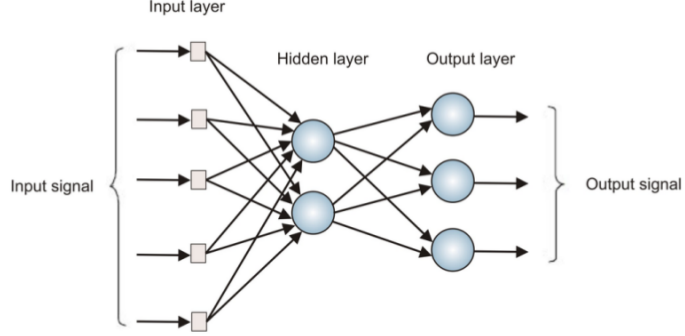
\includegraphics[width=0.8\textwidth]{nn.png}
\caption{\label{fig:nn}Structure of a Multi-layer Perceptron \cite{nn}.}
\end{figure}

Multilayer perceptron with single layer can solve a wide variety of problems. The weights can initially be assumed randomly and then the network can be trained by backpropagation \cite{bp}. The implementation given in \textit{scikitlearn} was used and the hyper-parameter values are given in Table~\ref{tab:nn1}. 

\begin{table}
\centering
\begin{tabular}{l|r}
hyper-parameter & values \\\hline
Train-Test split & 90:10 \\
Hidden-layer dimensions & 500, 100 \\
Activation Function & Relu \\
Optimizer & Adam \\
Regularization Coefficient & 0.0001 \\
Batch Size & 200 \\
Learning Rate & 0.001 (constant) \\
Maximum Iterations & 200 \\
Tolerance & 1e-4
\end{tabular}
\caption{\label{tab:nn1}Hyper-parameters for MLP setup.}
\end{table}

\subsection{Support Vector Regression}
Support Vector Machine can be applied not only to the classification problems but also to the regression problems. Similar to classification, the basic aim is to optimize the generalization bounds for regression \cite{svr}. It uses an epsilon intensive loss function which ignores errors that are situated within the certain distance of the true value. Figure~\ref{fig:sv} below shows an example of one-dimensional linear regression function with epsilon intensive band. The variables measure the cost of the errors on the training points. The error is zero for all points inside the epsilon band. SV algorithm can be made nonlinear by simply pre-processing the training patterns with kernel functions. In the nonlinear setting, the optimization problem corresponds to finding the flattest function in feature space, not in input space. The implementation given in \textit{scikitlearn} was used and the hyper-parameter values are given in Table~\ref{tab:svr1}.

\begin{figure}
\centering
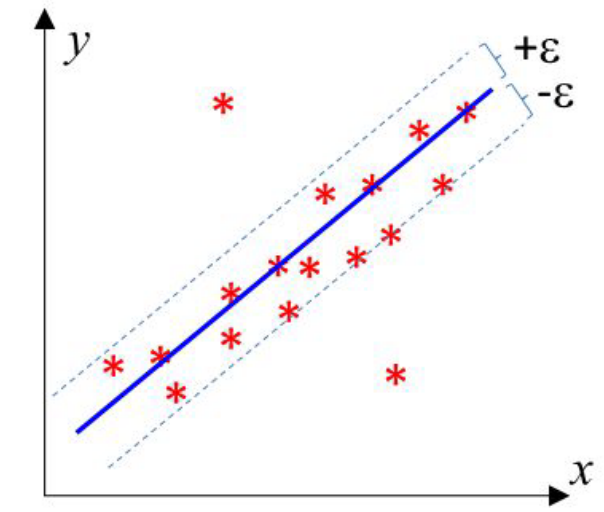
\includegraphics[width=0.5\textwidth]{sv.png}
\caption{\label{fig:sv}Linear regression function with epsilon insensitive band \cite{svr}.}
\end{figure} 

\begin{table}
\centering
\begin{tabular}{l|r}
hyper-parameter & values \\\hline
Train-Test split & 90:10 \\
C & 1.0 \\
Epsilon & 0.1 \\
Kernel & RBF \\
Tolerance & 1e-3
\end{tabular}
\caption{\label{tab:svr1}Hyper-parameters for SVR setup.}
\end{table}

\section{Evaluation and Analysis}

\subsection{Datasets}
Two TEDx videos were used of lengths 624 seconds and 719 seconds. Then acoustic feature datasets obtained were of dimensions 6373x620 and 6373x714. Feature selection reduced the dataset size to \textit{n}x620 and \textit{n}x714 where \textit{n} was a hyper-parameter. The eyeblink data had dimensions 620x1 and 714x1. 

\subsection{Evaluation Metric}
The $R^2$ score was used as a performance metric for the learning algorithms used in the last experiment. The coefficient $R^2$ is defined as: 
$$R^2 = (1 - \frac{u}{v})$$

, where $u$ is the residual sum of squares and $v$ is the total sum of squares. The best possible score is 1.0 and it can be negative (because the model can be arbitrarily worse). A constant model that always predicts the expected value of target, disregarding the input features, would get a $R^2$ score of 0.0.

\subsection{Results}
The $R^2$ results for both the MLP and SVR setups were obtained in the first four experiments mentioned below. Four different experiments were conducted with the feature selection and learning methods. In the fifth experiment, the relevant acoustic features were determined. Since only correlation analysis gave good results, relevant features were determined for this feature selection.

\subsubsection{Full Audience and Feature Selection with Eigen-analysis}

The follwing $R^2$ results were obtained for given reduced acoustic dataset sizes. Table~\ref{tab:carol1} gives results for Carol TEDx video and Table~\ref{tab:simon1} for Simon TEDx video. Figure~\ref{fig:f1} shows the plot for the best result obtained here.

\begin{table}
\centering
\begin{tabular}{ |p{3cm}||p{3cm}|p{3cm}|p{3cm}|  }
 \hline
 \multicolumn{3}{|c|}{$R^2 scores$} \\
 \hline
 Dataset Size &MLP &SVR\\
 \hline
 10 & -0.13 &-0.006\\
 20 & 0.12 & 0.08\\
 50 & -0.09 & 0.20\\
 100 & -0.90 & 0.16\\
 200 & -1.52 & 0.24\\
 \hline
\end{tabular}
\caption{\label{tab:carol1}Results for Carol Video.}
\end{table}

\begin{table}
\centering
\begin{tabular}{ |p{3cm}||p{3cm}|p{3cm}|p{3cm}|  }
 \hline
 \multicolumn{3}{|c|}{$R^2 scores$} \\
 \hline
 Dataset Size &MLP &SVR\\
 \hline
 10 & -0.18 &-0.12\\
 20 & 0.29 & 0.16\\
 50 & 0.03 & 0.13\\
 100 & -0.30 & 0.19\\
 200 & -0.28 & 0.25\\
 \hline
\end{tabular}
\caption{\label{tab:simon1}Results for Simon Video.}
\end{table}

\begin{figure}
\centering
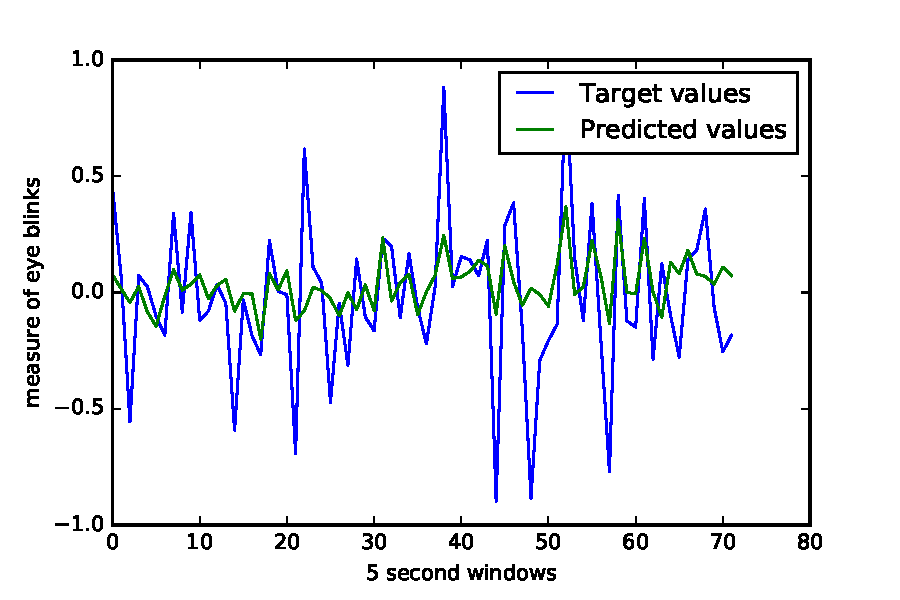
\includegraphics[width=0.4\textwidth]{f1.pdf}
\caption{\label{fig:f1}Plot for Simon Video with SVR and size 200.}
\end{figure} 

\subsubsection{Full Audience and Feature Selection with Correlation-analysis}

The follwing $R^2$ results were obtained for given reduced acoustic dataset sizes. Table~\ref{tab:carol2} gives results for Carol TEDx video and Table~\ref{tab:simon2} for Simon TEDx video. Figure~\ref{fig:f2} shows the plot for the best result obtained here.

\begin{table}
\centering
\begin{tabular}{ |p{3cm}||p{3cm}|p{3cm}|p{3cm}|  }
 \hline
 \multicolumn{3}{|c|}{$R^2 scores$} \\
 \hline
 Dataset Size &MLP &SVR\\
 \hline
 10 & 0.23 & 0.11\\
 20 & 0.47 & 0.44\\
 50 & 0.38 & 0.43\\
 100 & 0.26 & 0.48\\
 200 & 0.19 & 0.44\\
 \hline
\end{tabular}
\caption{\label{tab:carol2}Results for Carol Video.}
\end{table}

\begin{table}
\centering
\begin{tabular}{ |p{3cm}||p{3cm}|p{3cm}|p{3cm}|  }
 \hline
 \multicolumn{3}{|c|}{$R^2 scores$} \\
 \hline
 Dataset Size &MLP &SVR\\
 \hline
 10 & 0.31 & 0.21\\
 20 & 0.48 & 0.40\\
 50 & 0.54 & 0.45\\
 100 & 0.48 & 0.52\\
 200 & 0.45 & 0.55\\
 \hline
\end{tabular}
\caption{\label{tab:simon2}Results for Simon Video.}
\end{table}

\begin{figure}
\centering
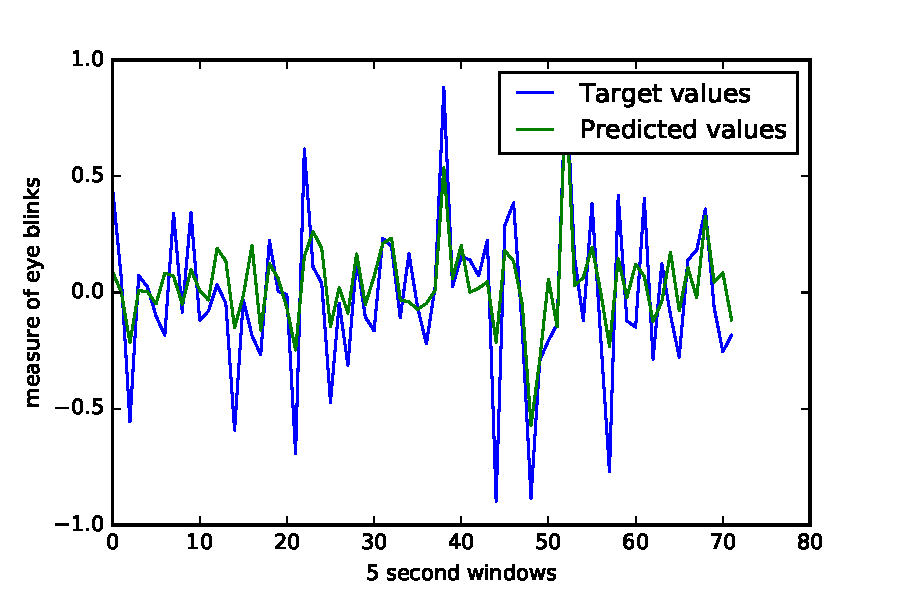
\includegraphics[width=0.4\textwidth]{f2.pdf}
\caption{\label{fig:f2}Plot for Simon Video with SVR and size 200.}
\end{figure} 

\subsubsection{Reduced Audience and Feature Selection with Eigen-analysis}

The follwing $R^2$ results were obtained for given reduced acoustic dataset sizes. Table~\ref{tab:carol3} gives results for Carol TEDx video and Table~\ref{tab:simon3} for Simon TEDx video. Figure~\ref{fig:f3} shows the plot for the best result obtained here.

\begin{table}
\centering
\begin{tabular}{ |p{3cm}||p{3cm}|p{3cm}|p{3cm}|  }
 \hline
 \multicolumn{3}{|c|}{$R^2 scores$} \\
 \hline
 Dataset Size &MLP &SVR\\
 \hline
 10 & -0.52 & 0.09\\
 20 & -0.03 & 0.28\\
 50 & -0.008 & 0.31\\
 100 & 0.03 & 0.32\\
 200 & -0.68 & 0.29\\
 \hline
\end{tabular}
\caption{\label{tab:carol3}Results for Carol Video.}
\end{table}

\begin{table}
\centering
\begin{tabular}{ |p{3cm}||p{3cm}|p{3cm}|p{3cm}|  }
 \hline
 \multicolumn{3}{|c|}{$R^2 scores$} \\
 \hline
 Dataset Size &MLP &SVR\\
 \hline
 10 & -0.32 & -0.114\\
 20 & 0.12 & 0.095\\
 50 & 0.26 & 0.14\\
 100 & 0.20 & 0.17\\
 200 & -0.17 & 0.16\\
 \hline
\end{tabular}
\caption{\label{tab:simon3}Results for Simon Video.}
\end{table}

\begin{figure}
\centering
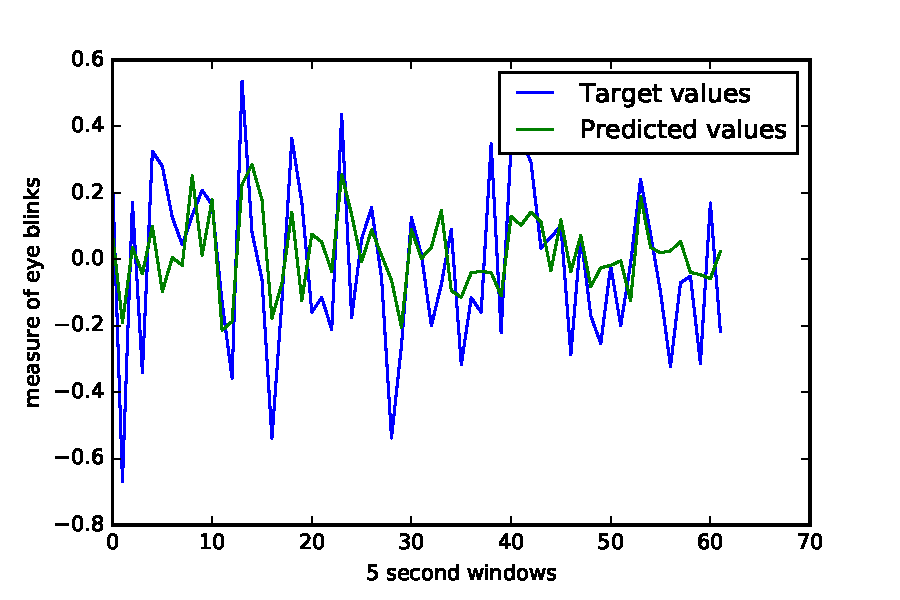
\includegraphics[width=0.4\textwidth]{f3.pdf}
\caption{\label{fig:f3}Plot for Carol Video with SVR and size 100.}
\end{figure} 

\subsubsection{Reduced Audience and Feature Selection with Correlation-analysis}

The follwing $R^2$ results were obtained for given reduced acoustic dataset sizes. Table~\ref{tab:carol4} gives results for Carol TEDx video and Table~\ref{tab:simon4} for Simon TEDx video. Figure~\ref{fig:f4} shows the plot for the best result obtained here.

\begin{table}
\centering
\begin{tabular}{ |p{3cm}||p{3cm}|p{3cm}|p{3cm}|  }
 \hline
 \multicolumn{3}{|c|}{$R^2 scores$} \\
 \hline
 Dataset Size &MLP &SVR\\
 \hline
 10 & 0.004 & 0.14\\
 20 & 0.34 & 0.40\\
 50 & 0.36 & 0.48\\
 100 & 0.39 & 0.51\\
 200 & 0.20 & 0.53\\
 \hline
\end{tabular}
\caption{\label{tab:carol4}Results for Carol Video.}
\end{table}

\begin{table}
\centering
\begin{tabular}{ |p{3cm}||p{3cm}|p{3cm}|p{3cm}|  }
 \hline
 \multicolumn{3}{|c|}{$R^2 scores$} \\
 \hline
 Dataset Size &MLP &SVR\\
 \hline
 10 & 0.27 & 0.34\\
 20 & 0.51 & 0.43\\
 50 & 0.47 & 0.52\\
 100 & 0.48 & 0.53\\
 200 & 0.51 & 0.57\\
 \hline
\end{tabular}
\caption{\label{tab:simon4}Results for Simon Video.}
\end{table}

\begin{figure}
\centering
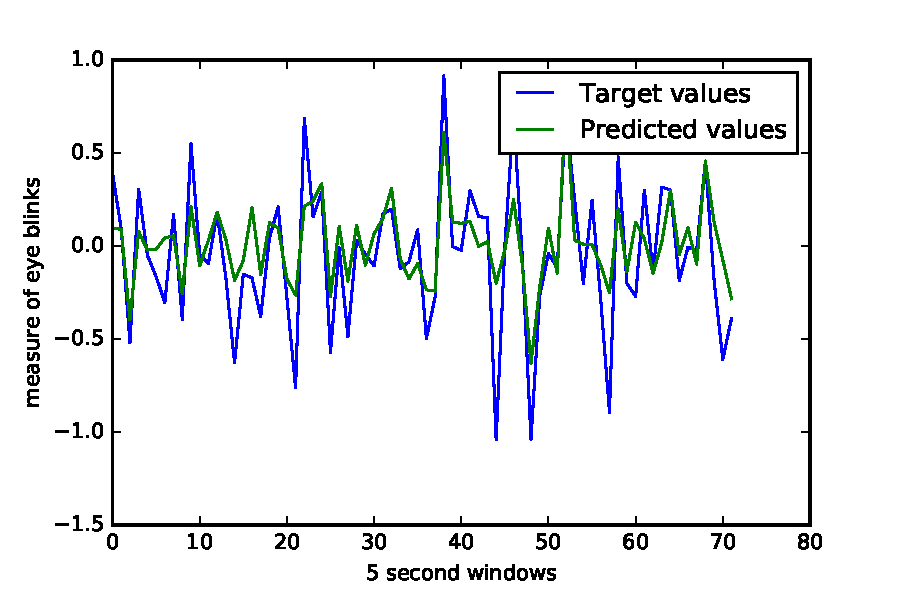
\includegraphics[width=0.4\textwidth]{f4.pdf}
\caption{\label{fig:f4}Plot for Simon Video with SVR and size 200.}
\end{figure} 

\subsubsection{Relevant Features with respect to Attention}
Only the correlation-analysis gave good results. Therefore the relevant features obtained through this feature selection were determined for both the full audience case and reduced one.

Top 10 features for Carol video with Full Audience:
\begin{itemize}
\item \verb|audspec_lengthL1norm_sma_stddev|:standard deviation of magnitude of the L1 norm of auditory spectrum and it was smoothed using an averaging filter with window length 3.
\item \verb|audSpec_Rfilt_sma[0]_range|:Rfilt means Relative Spectral Transform (RASTA)-style filtered. This means range of 0th Rfilt of auditory spectrum and it was smoothed using an averaging filter with window length 3.
\item \verb|audSpec_Rfilt_sma[19]_percentile1.0|:Rfilt means Relative Spectral Transform (RASTA)-style filtered. Percentile1.0 is the outlier-robust minimum value of the contour, represented by the 1 percentile. This means percentile1.0 of 19th Rfilt of auditory spectrum and it was smoothed using an averaging filter with window length 3.
\item \verb|audSpec_Rfilt_sma[24]_range|:Rfilt means Relative Spectral Transform (RASTA)-style filtered. This means range of 24th Rfilt of auditory spectrum and it was smoothed using an averaging filter with window length 3.
\item \verb|audSpec_Rfilt_sma[25]_percentile1.0|:Rfilt means Relative Spectral Transform (RASTA)-style filtered. Percentile1.0 is the outlier-robust minimum value of the contour, represented by the 1 percentile. This means percentile1.0 of 25th Rfilt of auditory spectrum and it was smoothed using an averaging filter with window length 3.
\item \verb|pcm_fftMag_spectralRollOff75.0_sma_leftctime|: The 75 ∗ 100 percent spectral roll-off point is determined as the frequency below which 75 ∗ 100 percent of the total signal energy fall. This means time during which the spectralRollOff75.0 of fast Fourier transformed pulse-code modulation has left curvature and it was smoothed using an averaging filter with window length 3.
\item \verb|mfcc_sma[2]_range|:range of 2nd mel-frequency cepstral coefficient and it was smoothed using an averaging filter with window length 3.
\item \verb|mfcc_sma[4]_percentile1.0|:Percentile1.0 is the outlier-robust minimum value of the contour, represented by the 1 percentile. This means percentile1.0 of 4th mel-frequency cepstral coefficient and it was smoothed using an averaging filter with window length 3.
\item \verb|mfcc_sma[8]_percentile99.0|:Percentile99.0 is the outlier-robust maximum value of the contour, represented by the 99 percentile. This means percentile99.0 of 8th mel-frequency cepstral coefficient and it was smoothed using an averaging filter with window length 3.
\item \verb|mfcc_sma_de[4]_range|:range of 4th mel-frequency cepstral coefficient and it was smoothed using an averaging filter with window length 3.
\end{itemize}

Top 10 features for Simon video with Full Audience:
\begin{itemize}
\item \verb|pcm_zcr_sma_percentile99.0|:Percentile99.0 is the outlier-robust maximum value of the contour, represented by the 99 percentile. This means percentile99.0 of zero-crossing rate of time signal and it was smoothed using an averaging filter with window length 3.
\item \verb|audspec_lengthL1norm_sma_de_range|:range of magnitude of the L1 norm of auditory spectrum and it was smoothed using an averaging filter with window length 3.
\item \verb|audSpec_Rfilt_sma[9]_range|:Rfilt means Relative Spectral Transform (RASTA)-style filtered. This means range of 9th Rfilt of auditory spectrum and it was smoothed using an averaging filter with window length 3.
\item \verb|audSpec_Rfilt_sma[15]_range|:Rfilt means Relative Spectral Transform (RASTA)-style filtered. This means range of 15th Rfilt of auditory spectrum and it was smoothed using an averaging filter with window length 3.
\item \verb|audSpec_Rfilt_sma[16]_pctlrange0-1|:Rfilt means Relative Spectral Transform (RASTA)-style filtered. This means 0-1 inter-percentile range of 16th Rfilt of auditory spectrum and it was smoothed using an averaging filter with window length 3.
\item \verb|pcm_fftMag_spectralRollOff25.0_sma_range|: The 25 ∗ 100 percent spectral roll-off point is determined as the frequency below which 25 ∗ 100 percent of the total signal energy fall. This means range of spectralRollOff25.0 of fast Fourier transformed pulse-code modulation and it was smoothed using an averaging filter with window length 3.
\item \verb|pcm_fftMag_spectralHarmonicity_sma_range|:A Harmonicity object represents the degree of acoustic periodicity, also called Harmonics-to-Noise Ratio (HNR). This means range of spectral harmonicity of fast Fourier transformed pulse-code modulation and it was smoothed using an averaging filter with window length 3.
\item \verb|audSpec_Rfilt_sma_de[8]_range|:Rfilt means Relative Spectral Transform (RASTA)-style filtered. This means range of 8th Rfilt of auditory spectrum and it was smoothed using an averaging filter with window length 3.
\item \verb|pcm_fftMag_spectralSlope_sma_peakRangeAbs|:absolute value of range of all values for spectral slope of fast Fourier transformed pulse-code modulation and it was smoothed using an averaging filter with window length 3.
\item \verb|audspec_lengthL1norm_sma_de_peakRangeAbs|:absolute value of range of all values for magnitude of the L1 norm of auditory spectrum and it was smoothed using an averaging filter with window length 3.
\end{itemize}

Top 10 features for Carol video with Reduced Audience:
\begin{itemize}
\item \verb|audspec_lengthL1norm_sma_quartile2|:$50th$ percentile of magnitude of the L1 norm of auditory spectrum and it was smoothed using an averaging filter with window length 3.
\item \verb|pcm_RMSenergy_sma_percentile99.0|:Percentile99.0 is the outlier-robust maximum value of the contour, represented by the 99 percentile. This means percentile99.0 of root-mean-square signal frame energy and it was smoothed using an averaging filter with window length 3.
\item \verb|pcm_RMSenergy_sma_pctlrange0-1|:This means 0-1 inter-percentile range of root-mean-square signal frame energy and it was smoothed using an averaging filter with window length 3.
\item \verb|audSpec_Rfilt_sma[20]_percentile1.0|:Rfilt means Relative Spectral Transform (RASTA)-style filtered. Percentile1.0 is the outlier-robust minimum value of the contour, represented by the 1 percentile. This means percentile1.0 of 20th Rfilt of auditory spectrum and it was smoothed using an averaging filter with window length 3.
\item \verb|mfcc_sma[1]_percentile99.0|:Percentile99.0 is the outlier-robust maximum value of the contour, represented by the 99 percentile. This means percentile99.0 of 1st mel-frequency cepstral coefficient and it was smoothed using an averaging filter with window length 3.
\item \verb|audSpec_Rfilt_sma_de[23]_percentile99.0|:Rfilt means Relative Spectral Transform (RASTA)-style filtered. Percentile99.0 is the outlier-robust maximum value of the contour, represented by the 99 percentile. This means percentile99.0 of 25th Rfilt of auditory spectrum and it was smoothed using an averaging filter with window length 3.
\item \verb|audSpec_Rfilt_sma[6]_meanRisingSlope|:meanRisingSlope is the mean of rising slopes, i.e. the slopes connecting a valley with the following peak. Rfilt means Relative Spectral Transform (RASTA)-style filtered. This means meanRisingSlope of 6th Rfilt of auditory spectrum and it was smoothed using an averaging filter with window length 3.
\item \verb|pcm_fftMag_spectralRollOff50.0_sma_minRangeRel|:The 50 ∗ 100 percent spectral roll-off point is determined as the frequency below which 50 ∗ 100 percent of the total signal energy fall. This means minimum value of relative range of spectralRollOff50.0 of fast Fourier transformed pulse-code modulation and it was smoothed using an averaging filter with window length 3.
\item \verb|audSpec_Rfilt_sma_de[21]_peakMeanAbs|:Rfilt means Relative Spectral Transform (RASTA)-style filtered. This means absolute value of mean of all values for 21th Rfilt of auditory spectrum and it was smoothed using an averaging filter with window length 3.
\item \verb|audSpec_Rfilt_sma_de[21]_peakMeanMeanDist|:Rfilt means Relative Spectral Transform (RASTA)-style filtered. This means mean of distance between peaks for 21th Rfilt of auditory spectrum and it was smoothed using an averaging filter with window length 3.
\end{itemize}

Top 10 features for Simon video with Reduced Audience:
\begin{itemize}
\item \verb|audSpec_Rfilt_sma[13]_range|:Rfilt means Relative Spectral Transform (RASTA)-style filtered. This means range of 13th Rfilt of auditory spectrum and it was smoothed using an averaging filter with window length 3.
\item \verb|audSpec_Rfilt_sma[23]_range|:Rfilt means Relative Spectral Transform (RASTA)-style filtered. This means range of 23th Rfilt of auditory spectrum and it was smoothed using an averaging filter with window length 3.
\item \verb|pcm_fftMag_spectralRollOff25.0_sma_percentile99.0|:Percentile99.0 is the outlier-robust maximum value of the contour, represented by the 99 percentile. The 25 ∗ 100 percent spectral roll-off point is determined as the frequency below which 25 ∗ 100 percent of the total signal energy fall. This means percentile99.0 of spectralRollOff25.0 of fast Fourier transformed pulse-code modulation and it was smoothed using an averaging filter with window length 3.
\item \verb|pcm_fftMag_spectralFlux_sma_range|:range of spectral flux of fast Fourier transformed pulse-code modulation and it was smoothed using an averaging filter with window length 3.
\item \verb|pcm_fftMag_spectralSkewness_sma_range|:Spectral skewness is a measure of the asymmetry of the spectral distribution around its centroid. This means range of spectral skewness of fast Fourier transformed pulse-code modulation and it was smoothed using an averaging filter with window length 3.
\item \verb|pcm_fftMag_psySharpness_sma_percentile1.0|:psySharpness is related to how much a sound’s spectrum is in the high end. Percentile1.0 is the outlier-robust minimum value of the contour, represented by the 1 percentile. This means percentile1.0 of psySharpness of fast Fourier transformed pulse-code modulation and it was smoothed using an averaging filter with window length 3.
\item \verb|mfcc_sma[6]_percentile1.0|:Percentile1.0 is the outlier-robust minimum value of the contour, represented by the 1 percentile. This means percentile1.0 of 6th mel-frequency cepstral coefficient and it was smoothed using an averaging filter with window length 3.
\item \verb|audSpec_Rfilt_sma_de[20]_range|:Rfilt means Relative Spectral Transform (RASTA)-style filtered. This means range of 20th Rfilt of auditory spectrum and it was smoothed using an averaging filter with window length 3.
\item \verb|pcm_fftMag_spectralFlux_sma_de_range|:delta of range of spectral flux of fast Fourier transformed pulse-code modulation and it was smoothed using an averaging filter with window length 3.
\item \verb|audSpec_Rfilt_sma_de[5]_stddevRisingSlope|:stddevRisingSlope is the standard deviation of rising slopes, i.e. the slopes connecting a valley with the following peak. Rfilt means Relative Spectral Transform (RASTA)-style filtered. This means stddevRisingSlope of 5th Rfilt of auditory spectrum and it was smoothed using an averaging filter with window length 3.
\end{itemize}

\section{Conclusion}

Best results were obtained using the correlation based feature selection for both the full audience and reduced audience case. For the full audience experiment, the best results were obtained for Simon video with SVR and correlation based feature selection of 200 features. Again for reduced dataset experiment, the best results were obtained for Simon video with SVR and correlation based feature selection of 200 features. The SVR learning method consistently out-performed the MLP method. 

The relevant audio features were also obtained for both the experiments. Future work can include further interpretation of the relevant features obtained. Also some other audio feature extraction methods can be explored. 


\begin{thebibliography}{9}
\bibitem{political} 
Zhang, John R., et al.
\textit{Correlating Speaker Gestures in Political Debates with Audience Engagement Measured via EEG}. 
Proceedings of the ACM International Conference on Multimedia. ACM, 2014.

\bibitem{opensmile} 
Eyben, Florian, Martin Wllmer, and Bjrn Schuller.
\textit{Opensmile: the munich versatile and fast open-source audio feature extractor}. 
Proceedings of the international conference on Multimedia. ACM, 2010.

\bibitem{compare} 
Schuller, Bjrn, et al.
\textit{The INTERSPEECH 2013 computational paralinguistics challenge: social signals, conflict, emotion, autism}. 
(2013).

\bibitem{audio} 
Eyben, Florian, et al.
\textit{The acoustics of eye contact: detecting visual attention from conversational audio cues}. 
Proceedings of the 6th workshop on Eye gaze in intelligent human machine interaction: gaze in multimodal interaction. ACM, 2013.

\bibitem{ffmpeg} 
Bellard, Fabrice, and M. Niedermayer.
\textit{FFmpeg}. 
http://ffmpeg.org (2012).

\bibitem{scikit} 
Pedregosa et al.
\textit{Scikit-learn: Machine Learning in Python}. 
JMLR 12, pp. 2825-2830, 2011.

\bibitem{nn} 
M.W.Gardener, S.R. Dorling.
\textit{ARTIFICIAL Neural Networks(The Multilayer perceptron)- A review of the applications in Atmospheric Sciences}. 
June 1998.

\bibitem{bp} 
Christopher Bishop.
\textit{Pattern Recognition and Machine Learning}. 
book, (2007).

\bibitem{svr} 
Alex J. Samola, Bernard S.
\textit{A tutorial on Support Vector Regression}. 
NeuroCOLT2 Technical Report NCR2, October 1998.

\end{thebibliography}

%\bibliography{references}

\end{document} to your LaTeX file where you want your
% title page.
%
%%%%%%%%%%%%%%%%%%%%%%%%%%%%%%%%%%%%%%%%%
%\title{Title page with logo}
%----------------------------------------------------------------------------------------
%	PACKAGES AND OTHER DOCUMENT CONFIGURATIONS
%----------------------------------------------------------------------------------------

\documentclass[12pt]{article}
\usepackage[english]{babel}
\usepackage[utf8x]{inputenc}
\usepackage{amsmath}
\usepackage{graphicx}
\usepackage[colorinlistoftodos]{todonotes}

\begin{document}

\begin{titlepage}

\newcommand{\HRule}{\rule{\linewidth}{0.5mm}} % Defines a new command for the horizontal lines, change thickness here

\center % Center everything on the page
 
%----------------------------------------------------------------------------------------
%	HEADING SECTIONS
%----------------------------------------------------------------------------------------

\textsc{\LARGE Columbia University}\\[1.5cm] % Name of your university/college
\textsc{\Large Project Report}\\[0.5cm] % Major heading such as course name
\textsc{\large COMS 6901}\\[0.5cm] % Minor heading such as course title

%----------------------------------------------------------------------------------------
%	TITLE SECTION
%----------------------------------------------------------------------------------------

\HRule \\[0.4cm]
{ \Large \bfseries Correlation of acoustic features of speakers with Audience Engagement}\\[0.5cm] % Title of your document
\HRule \\[0.5cm]
 
%----------------------------------------------------------------------------------------
%	AUTHOR SECTION
%----------------------------------------------------------------------------------------

\begin{minipage}{0.4\textwidth}
\begin{flushleft} \large
\emph{Author:}\\
Animesh Sharma % Your name
\end{flushleft}
\end{minipage}
~
\begin{minipage}{0.4\textwidth}
\begin{flushright} \large
\emph{Supervisor:} \\
Dr. John Kender % Supervisor's Name
\end{flushright}
\end{minipage}\\[2cm]

% If you don't want a supervisor, uncomment the two lines below and remove the section above
%\Large \emph{Author:}\\
%John \textsc{Smith}\\[3cm] % Your name

%----------------------------------------------------------------------------------------
%	DATE SECTION
%----------------------------------------------------------------------------------------

{\large \today}\\[1cm] % Date, change the \today to a set date if you want to be precise

%----------------------------------------------------------------------------------------
%	LOGO SECTION
%----------------------------------------------------------------------------------------


\includegraphics{CU_logo.jpg}\\[0.5cm] % Include a department/university logo - this will require the graphicx package
 
%----------------------------------------------------------------------------------------

\vfill % Fill the rest of the page with whitespace

\end{titlepage}

\begin{abstract}
In this work, we investigate the extent to which the acoustic features of speakers are correlated to the audience engagement. The number of eyeblinks in a particular time period was taken as a measure of engagement of audience and the acoustic feature set of size 6373 was obtained for two different TEDx videos- Simon and Carol, with the help of OpenSmile software. Then eigen-analysis and mutual info regression based correlation analysis were used for feature selection in case of audio feature set. In order to determine the extent to which the acoustic features are correlated with the attention signal, two learning algorithms- Multi-layer Perceptron (MLP) and Support Vector Regression (SVR), were used to predict the attention signal with the acoustic feature set being used as input to the network. The best $R^2$ score of 0.55 was obtained for the correlation based analysis of Simon video with Support Vector Regression and acoustic feature set of size 200. Then the anomalies in audience, which were previously being handled through Z-score, were removed and all the experiments were performed again. This time the best result was 0.57 for Simon video with correlation based analysis and Support Vector Regression. The audio features most correlated with eyeblink data were also listed for both cases with feature selection based on correlation analysis.
\end{abstract}

\clearpage

\tableofcontents

\clearpage

\section{Introduction}

This project is based on the work done by Zhang et al. \cite{political}. in which the authors propose that certain speaker gestures can convey important information regarding audience engagement. Two TEDx videos, labeled Simon and Carol, were used for this project and it was studied whether certain acoustic features have more influence on the audience engagement. This work is useful in determining whether audience engagement can be improved with the help of the observed acoustic features. The acoustic features most correlated with the audience engagement can help instructors and speakers in further engaging their audience. The eyeblink data was used as a measure of the audience engagement based on the premise that the subject tends to pay more attention when the number of eyeblinks are less for that time period. There were 28 subjects for both the videos and the number of eyeblinks for a 5 second window were obtained for the audience as a whole by taking the mean for that time period. The acoustic feature dataset of size 6373 was obtained using OpenSmile \cite{opensmile}. software and this dataset was then used as input to the learning algorithms. This acoustic feature set, known as ComParE feature set \cite{compare}, was given by Eybet et al \cite{audio} and they are functionals of acoustic low level descriptors (LLDs). Then feature selection was done for the audio feature set so as to evaluate the performance of the learning algorithms only on the relevant features and to filter out the noise. The learning algorithms were used to determine whether the attention signal can be predicted with acoustic signal as input. The performance of the learning algorithm give a sense of the importance of audio features in determing the audience engagement. Furthermore, the important audio features determined by correlating them with attention signal can also be listed so that it can be known which audio features out of the feature set of size 6373 influence the attention signal most. Predicting the attention signal is a regression problem and two different learning algorithms were used for the same. One important issue with this task was handling the anomalies present in the eyeblink dataset of audience. Some of the eyeblink recordings of the subjects were corrupted in the sense that there were two many eyeblinks in certain 5 second windows. These anomalies were handled by taking Z-scores of the recordings in first case and afterwards removing them in the second. All the steps were repeated for both the cases.

\section{Problem Formulation}

Two different datasets- eyeblink dataset and acoustic feature dataset, were prepared for this work and then subsequent analysis was done for determining how much one is correlated with the other.The whole project pipeline has 5 subsections and these were executed in-order to obtain the final result. The following contributions were made in this work:
\begin{enumerate}
\item The eyeblink data was cleaned and pre-processed to get an attention signal for the audience. The experiments were conducted first for all the 28 subjects in audience and then the anomalies were removed and the experiments were repeated for 17 subjects. The outlier subjects were removed on the criteria that for these subjects, the number of eyeblinks in a 5 second window was too high for a human being.
\item The acoustic feature dataset was prepared for the two TEDx videos for 5 second windows using OpenSmile software. The audio was stripped off from the video file and 5 second windows were obtained using ffmpeg wrapper \cite{ffmpeg}. 
\item The acoustic feature set of size 6373 was reduced to sizes 10, 20, 50, 100 and 200 using eigenanalysis and mutual information based correlation analysis. The scikit-learn library in Python \cite{scikit} was used for this feature selection. The reduced feature set in eigenanalysis was further preprocessed using Z-score method.
\item Then it was determined whether its possible to predict the attention of the audience with reduced acoustic feature set. Two different learning algorithms were used - Neural Networks and Support Vector Regression. The scikit-learn was again used here and the network settings for both the methods are defined in subsequent sections.
\item The different acoustic features obtained for both the full audience and the reduced audience were also listed and the meaning of these features was obtained so that it can be determined which characteristics of a person's speech are helpful in capturing attention of the audience.  
\end{enumerate}

\section{Proposed Method}
\label{sec:methods}

The following subsections define the different submodules executed for obtaining the final result given in this work. 

\subsection{Eyeblink data cleaning and preprocessing}

The raw data was in xls format and there were many redundant columns in it. The format was converted to csv. Multiple scripts in python were written for different preprocessing tasks. Only the follwing columns were retained- \verb|CURRENT_FIX_LABEL| column which gives the fixation timestamp and the \verb|NEXT_SAC_CONTAINS_BLINK| column which gives boolean values as to whether this section contains eyeblink or not. The data of the fixation column was converted to integer values and then the number of eyeblinks in a 5 second window was obtained. The Z-score values were obtained so as to normalize the eyeblink data with respect to each subject individually. Finally the mean of the eyeblink data for the audience was taken for each 5 second window.

\subsection{Handling Outliers in Eyeblink dataset}

For the first experiment, just the Z-score values were obtained for all the subjects. It was done so as to diffuse the effect of the outliers. There were 28 subjects for both the Simon and Carol video.

For the second experiment, the anomalies were removed for both the Simon and Carol videos. For the Carol video, the following subjects were removed with the given reasons:
\begin{itemize}
\item \verb|jc1_carol|: consistent eyeblinks of 6 or 5
\item \verb|jhh1_carol|, \verb|msb1_carol|: consistently high eyeblinks of 10
\item \verb|jy1_carol|, \verb|pp1_carol|, \verb|rn1_carol|: no eyeblinks at all (0 or 1)
\item \verb|pc1_carol|: lots of 10 at the end of the video
\item \verb|sa1_carol|, \verb|sd2_carol|, \verb|sw1_carol|, \verb|ys1_carol|: consistently high eyeblinks
\end{itemize}
\clearpage
For the Simon video, the following subjects were removed with the given reasons:
\begin{itemize}
\item \verb|jg1_simon|, \verb|pp1_simon|, \verb|rn1_simon|, \verb|jy1_simon|: no eyeblinks at all (0 or 1)
\item \verb|sa1_simon|, \verb|jc1_simon|, \verb|sd2_simon|, \verb|klt1_simon|, \verb|azz1_simon|, \verb|ys1_simon|, \verb|jhh1_simon|: consistently high eyeblinks
\end{itemize}

\subsection{Acoustic Feature Set}
The audio was extracted from the video files in \textit{mp3} format and then it was converted to \textit{wav} format using ffmpeg wrapper. Then a script in \textit{Ruby} was written to obtain 5 second windows for both the TEDx files and the offset was taken as 1 second here. Finally the ComParE audio feature set of size 6373 was obtained using OpenSmile and the output format was \textit{csv}.

The length of the Carol video was 624 seconds and therefore 620 fragments were obtained for this file. Similarly, 714 fragments were obtained for the Simon video with length 718 seconds.

\subsection{Feature Selection for Acoustic Feature Set}
Two different methods were used for reducing the size of the ComParE dataset obtained using OpenSmile. First the size was reduced using Eigenanalysis. The \textit{sklearn} package present in \textit{Python} was used here to reduce the dataset size to 10, 20, 50, 100 and 200. Then the values were normalized using Z-score method.

For the second method, correlation with the eyeblink data was used to select only \textit{n} features out of the 6373 available so that the selected features have highest correlation values. The method used here to calculate the correlation values was \textit{mutual info regression} present in \textit{sklearn} package. The reduced dataset sizes were again 10, 20, 50, 100 and 200 and the predefined method \textit{SelectKBest} available in \textit{scikitlearn} was used.

\subsection{Neural Networks}
A Multi-layer perceptron is a network of simple neurons called Perceptron. Each neuron computes the output which is some linear or usually a non-linear function of the linear combination of the input and the weights including the bias. A simple neuron has mapping limitations and thus a number or layers with a large number of neurons are used. The input neuron layer represents each instance which is fed to the hidden layer. The hidden layer computes the output depending on the input it receives, the corresponding weights and the activation function which is then fed to the output layer \cite{nn}. Thus the input signal propagates the network layer by layer. The number of the layers depends on the structure of the network. Figure~\ref{fig:nn} shows the structure of a multi-layer perceptron.

\begin{figure}
\centering
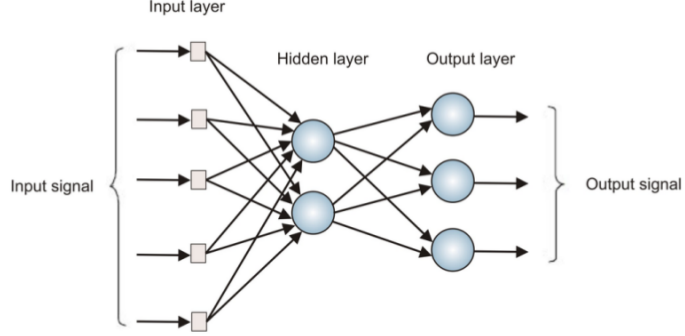
\includegraphics[width=0.8\textwidth]{nn.png}
\caption{\label{fig:nn}Structure of a Multi-layer Perceptron \cite{nn}.}
\end{figure}

Multilayer perceptron with single layer can solve a wide variety of problems. The weights can initially be assumed randomly and then the network can be trained by backpropagation \cite{bp}. The implementation given in \textit{scikitlearn} was used and the hyper-parameter values are given in Table~\ref{tab:nn1}. 

\begin{table}
\centering
\begin{tabular}{l|r}
hyper-parameter & values \\\hline
Train-Test split & 90:10 \\
Hidden-layer dimensions & 500, 100 \\
Activation Function & Relu \\
Optimizer & Adam \\
Regularization Coefficient & 0.0001 \\
Batch Size & 200 \\
Learning Rate & 0.001 (constant) \\
Maximum Iterations & 200 \\
Tolerance & 1e-4
\end{tabular}
\caption{\label{tab:nn1}Hyper-parameters for MLP setup.}
\end{table}

\subsection{Support Vector Regression}
Support Vector Machine can be applied not only to the classification problems but also to the regression problems. Similar to classification, the basic aim is to optimize the generalization bounds for regression \cite{svr}. It uses an epsilon intensive loss function which ignores errors that are situated within the certain distance of the true value. Figure~\ref{fig:sv} below shows an example of one-dimensional linear regression function with epsilon intensive band. The variables measure the cost of the errors on the training points. The error is zero for all points inside the epsilon band. SV algorithm can be made nonlinear by simply pre-processing the training patterns with kernel functions. In the nonlinear setting, the optimization problem corresponds to finding the flattest function in feature space, not in input space. The implementation given in \textit{scikitlearn} was used and the hyper-parameter values are given in Table~\ref{tab:svr1}.

\begin{figure}
\centering
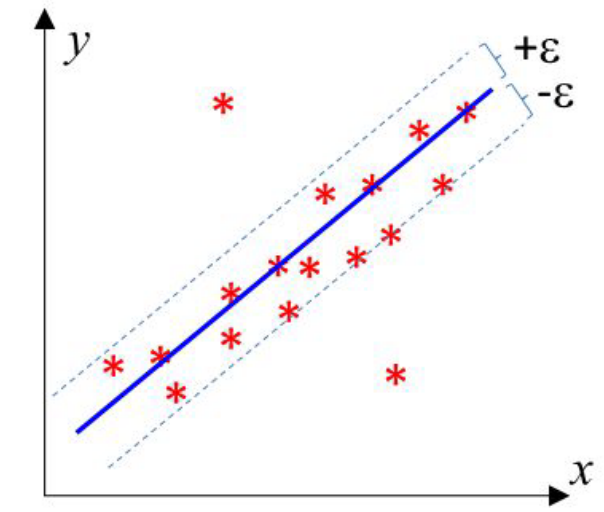
\includegraphics[width=0.5\textwidth]{sv.png}
\caption{\label{fig:sv}Linear regression function with epsilon insensitive band \cite{svr}.}
\end{figure} 

\begin{table}
\centering
\begin{tabular}{l|r}
hyper-parameter & values \\\hline
Train-Test split & 90:10 \\
C & 1.0 \\
Epsilon & 0.1 \\
Kernel & RBF \\
Tolerance & 1e-3
\end{tabular}
\caption{\label{tab:svr1}Hyper-parameters for SVR setup.}
\end{table}

\section{Evaluation and Analysis}

\subsection{Datasets}
Two TEDx videos were used of lengths 624 seconds and 719 seconds. Then acoustic feature datasets obtained were of dimensions 6373x620 and 6373x714. Feature selection reduced the dataset size to \textit{n}x620 and \textit{n}x714 where \textit{n} was a hyper-parameter. The eyeblink data had dimensions 620x1 and 714x1. 

\subsection{Evaluation Metric}
The $R^2$ score was used as a performance metric for the learning algorithms used in the last experiment. The coefficient $R^2$ is defined as: 
$$R^2 = (1 - \frac{u}{v})$$

, where $u$ is the residual sum of squares and $v$ is the total sum of squares. The best possible score is 1.0 and it can be negative (because the model can be arbitrarily worse). A constant model that always predicts the expected value of target, disregarding the input features, would get a $R^2$ score of 0.0.

\subsection{Results}
The $R^2$ results for both the MLP and SVR setups were obtained in the first four experiments mentioned below. Four different experiments were conducted with the feature selection and learning methods. In the fifth experiment, the relevant acoustic features were determined. Since only correlation analysis gave good results, relevant features were determined for this feature selection.

\subsubsection{Full Audience and Feature Selection with Eigen-analysis}

The follwing $R^2$ results were obtained for given reduced acoustic dataset sizes. Table~\ref{tab:carol1} gives results for Carol TEDx video and Table~\ref{tab:simon1} for Simon TEDx video. Figure~\ref{fig:f1} shows the plot for the best result obtained here.

\begin{table}
\centering
\begin{tabular}{ |p{3cm}||p{3cm}|p{3cm}|p{3cm}|  }
 \hline
 \multicolumn{3}{|c|}{$R^2 scores$} \\
 \hline
 Dataset Size &MLP &SVR\\
 \hline
 10 & -0.13 &-0.006\\
 20 & 0.12 & 0.08\\
 50 & -0.09 & 0.20\\
 100 & -0.90 & 0.16\\
 200 & -1.52 & 0.24\\
 \hline
\end{tabular}
\caption{\label{tab:carol1}Results for Carol Video.}
\end{table}

\begin{table}
\centering
\begin{tabular}{ |p{3cm}||p{3cm}|p{3cm}|p{3cm}|  }
 \hline
 \multicolumn{3}{|c|}{$R^2 scores$} \\
 \hline
 Dataset Size &MLP &SVR\\
 \hline
 10 & -0.18 &-0.12\\
 20 & 0.29 & 0.16\\
 50 & 0.03 & 0.13\\
 100 & -0.30 & 0.19\\
 200 & -0.28 & 0.25\\
 \hline
\end{tabular}
\caption{\label{tab:simon1}Results for Simon Video.}
\end{table}

\begin{figure}
\centering
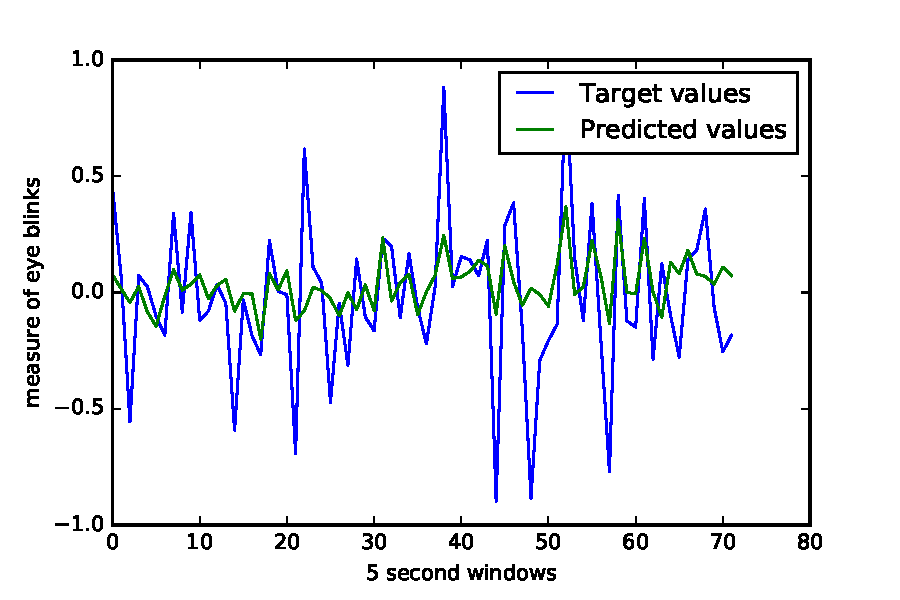
\includegraphics[width=0.4\textwidth]{f1.pdf}
\caption{\label{fig:f1}Plot for Simon Video with SVR and size 200.}
\end{figure} 

\subsubsection{Full Audience and Feature Selection with Correlation-analysis}

The follwing $R^2$ results were obtained for given reduced acoustic dataset sizes. Table~\ref{tab:carol2} gives results for Carol TEDx video and Table~\ref{tab:simon2} for Simon TEDx video. Figure~\ref{fig:f2} shows the plot for the best result obtained here.

\begin{table}
\centering
\begin{tabular}{ |p{3cm}||p{3cm}|p{3cm}|p{3cm}|  }
 \hline
 \multicolumn{3}{|c|}{$R^2 scores$} \\
 \hline
 Dataset Size &MLP &SVR\\
 \hline
 10 & 0.23 & 0.11\\
 20 & 0.47 & 0.44\\
 50 & 0.38 & 0.43\\
 100 & 0.26 & 0.48\\
 200 & 0.19 & 0.44\\
 \hline
\end{tabular}
\caption{\label{tab:carol2}Results for Carol Video.}
\end{table}

\begin{table}
\centering
\begin{tabular}{ |p{3cm}||p{3cm}|p{3cm}|p{3cm}|  }
 \hline
 \multicolumn{3}{|c|}{$R^2 scores$} \\
 \hline
 Dataset Size &MLP &SVR\\
 \hline
 10 & 0.31 & 0.21\\
 20 & 0.48 & 0.40\\
 50 & 0.54 & 0.45\\
 100 & 0.48 & 0.52\\
 200 & 0.45 & 0.55\\
 \hline
\end{tabular}
\caption{\label{tab:simon2}Results for Simon Video.}
\end{table}

\begin{figure}
\centering
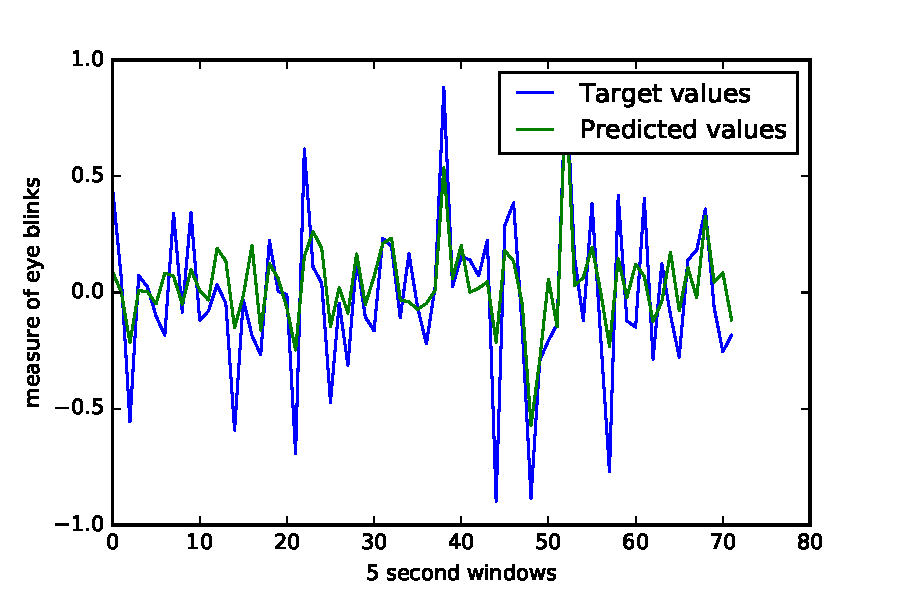
\includegraphics[width=0.4\textwidth]{f2.pdf}
\caption{\label{fig:f2}Plot for Simon Video with SVR and size 200.}
\end{figure} 

\subsubsection{Reduced Audience and Feature Selection with Eigen-analysis}

The follwing $R^2$ results were obtained for given reduced acoustic dataset sizes. Table~\ref{tab:carol3} gives results for Carol TEDx video and Table~\ref{tab:simon3} for Simon TEDx video. Figure~\ref{fig:f3} shows the plot for the best result obtained here.

\begin{table}
\centering
\begin{tabular}{ |p{3cm}||p{3cm}|p{3cm}|p{3cm}|  }
 \hline
 \multicolumn{3}{|c|}{$R^2 scores$} \\
 \hline
 Dataset Size &MLP &SVR\\
 \hline
 10 & -0.52 & 0.09\\
 20 & -0.03 & 0.28\\
 50 & -0.008 & 0.31\\
 100 & 0.03 & 0.32\\
 200 & -0.68 & 0.29\\
 \hline
\end{tabular}
\caption{\label{tab:carol3}Results for Carol Video.}
\end{table}

\begin{table}
\centering
\begin{tabular}{ |p{3cm}||p{3cm}|p{3cm}|p{3cm}|  }
 \hline
 \multicolumn{3}{|c|}{$R^2 scores$} \\
 \hline
 Dataset Size &MLP &SVR\\
 \hline
 10 & -0.32 & -0.114\\
 20 & 0.12 & 0.095\\
 50 & 0.26 & 0.14\\
 100 & 0.20 & 0.17\\
 200 & -0.17 & 0.16\\
 \hline
\end{tabular}
\caption{\label{tab:simon3}Results for Simon Video.}
\end{table}

\begin{figure}
\centering
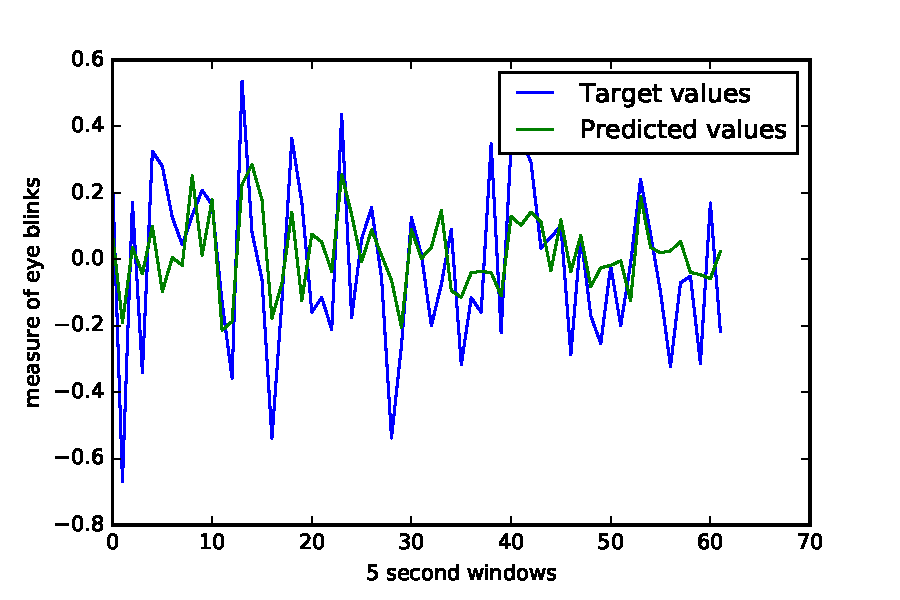
\includegraphics[width=0.4\textwidth]{f3.pdf}
\caption{\label{fig:f3}Plot for Carol Video with SVR and size 100.}
\end{figure} 

\subsubsection{Reduced Audience and Feature Selection with Correlation-analysis}

The follwing $R^2$ results were obtained for given reduced acoustic dataset sizes. Table~\ref{tab:carol4} gives results for Carol TEDx video and Table~\ref{tab:simon4} for Simon TEDx video. Figure~\ref{fig:f4} shows the plot for the best result obtained here.

\begin{table}
\centering
\begin{tabular}{ |p{3cm}||p{3cm}|p{3cm}|p{3cm}|  }
 \hline
 \multicolumn{3}{|c|}{$R^2 scores$} \\
 \hline
 Dataset Size &MLP &SVR\\
 \hline
 10 & 0.004 & 0.14\\
 20 & 0.34 & 0.40\\
 50 & 0.36 & 0.48\\
 100 & 0.39 & 0.51\\
 200 & 0.20 & 0.53\\
 \hline
\end{tabular}
\caption{\label{tab:carol4}Results for Carol Video.}
\end{table}

\begin{table}
\centering
\begin{tabular}{ |p{3cm}||p{3cm}|p{3cm}|p{3cm}|  }
 \hline
 \multicolumn{3}{|c|}{$R^2 scores$} \\
 \hline
 Dataset Size &MLP &SVR\\
 \hline
 10 & 0.27 & 0.34\\
 20 & 0.51 & 0.43\\
 50 & 0.47 & 0.52\\
 100 & 0.48 & 0.53\\
 200 & 0.51 & 0.57\\
 \hline
\end{tabular}
\caption{\label{tab:simon4}Results for Simon Video.}
\end{table}

\begin{figure}
\centering
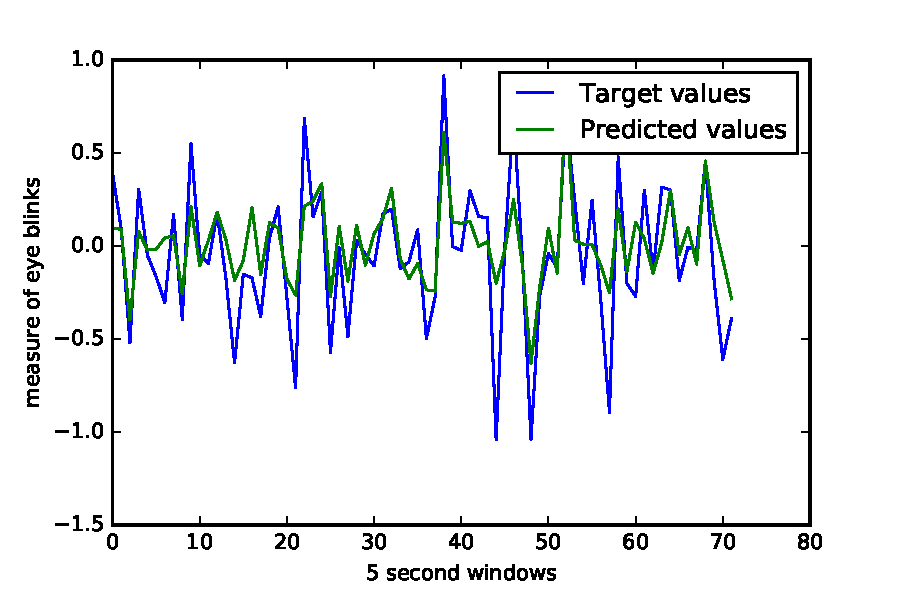
\includegraphics[width=0.4\textwidth]{f4.pdf}
\caption{\label{fig:f4}Plot for Simon Video with SVR and size 200.}
\end{figure} 

\subsubsection{Relevant Features with respect to Attention}
Only the correlation-analysis gave good results. Therefore the relevant features obtained through this feature selection were determined for both the full audience case and reduced one.

Top 10 features for Carol video with Full Audience:
\begin{itemize}
\item \verb|audspec_lengthL1norm_sma_stddev|:standard deviation of magnitude of the L1 norm of auditory spectrum and it was smoothed using an averaging filter with window length 3.
\item \verb|audSpec_Rfilt_sma[0]_range|:Rfilt means Relative Spectral Transform (RASTA)-style filtered. This means range of 0th Rfilt of auditory spectrum and it was smoothed using an averaging filter with window length 3.
\item \verb|audSpec_Rfilt_sma[19]_percentile1.0|:Rfilt means Relative Spectral Transform (RASTA)-style filtered. Percentile1.0 is the outlier-robust minimum value of the contour, represented by the 1 percentile. This means percentile1.0 of 19th Rfilt of auditory spectrum and it was smoothed using an averaging filter with window length 3.
\item \verb|audSpec_Rfilt_sma[24]_range|:Rfilt means Relative Spectral Transform (RASTA)-style filtered. This means range of 24th Rfilt of auditory spectrum and it was smoothed using an averaging filter with window length 3.
\item \verb|audSpec_Rfilt_sma[25]_percentile1.0|:Rfilt means Relative Spectral Transform (RASTA)-style filtered. Percentile1.0 is the outlier-robust minimum value of the contour, represented by the 1 percentile. This means percentile1.0 of 25th Rfilt of auditory spectrum and it was smoothed using an averaging filter with window length 3.
\item \verb|pcm_fftMag_spectralRollOff75.0_sma_leftctime|: The 75 ∗ 100 percent spectral roll-off point is determined as the frequency below which 75 ∗ 100 percent of the total signal energy fall. This means time during which the spectralRollOff75.0 of fast Fourier transformed pulse-code modulation has left curvature and it was smoothed using an averaging filter with window length 3.
\item \verb|mfcc_sma[2]_range|:range of 2nd mel-frequency cepstral coefficient and it was smoothed using an averaging filter with window length 3.
\item \verb|mfcc_sma[4]_percentile1.0|:Percentile1.0 is the outlier-robust minimum value of the contour, represented by the 1 percentile. This means percentile1.0 of 4th mel-frequency cepstral coefficient and it was smoothed using an averaging filter with window length 3.
\item \verb|mfcc_sma[8]_percentile99.0|:Percentile99.0 is the outlier-robust maximum value of the contour, represented by the 99 percentile. This means percentile99.0 of 8th mel-frequency cepstral coefficient and it was smoothed using an averaging filter with window length 3.
\item \verb|mfcc_sma_de[4]_range|:range of 4th mel-frequency cepstral coefficient and it was smoothed using an averaging filter with window length 3.
\end{itemize}

Top 10 features for Simon video with Full Audience:
\begin{itemize}
\item \verb|pcm_zcr_sma_percentile99.0|:Percentile99.0 is the outlier-robust maximum value of the contour, represented by the 99 percentile. This means percentile99.0 of zero-crossing rate of time signal and it was smoothed using an averaging filter with window length 3.
\item \verb|audspec_lengthL1norm_sma_de_range|:range of magnitude of the L1 norm of auditory spectrum and it was smoothed using an averaging filter with window length 3.
\item \verb|audSpec_Rfilt_sma[9]_range|:Rfilt means Relative Spectral Transform (RASTA)-style filtered. This means range of 9th Rfilt of auditory spectrum and it was smoothed using an averaging filter with window length 3.
\item \verb|audSpec_Rfilt_sma[15]_range|:Rfilt means Relative Spectral Transform (RASTA)-style filtered. This means range of 15th Rfilt of auditory spectrum and it was smoothed using an averaging filter with window length 3.
\item \verb|audSpec_Rfilt_sma[16]_pctlrange0-1|:Rfilt means Relative Spectral Transform (RASTA)-style filtered. This means 0-1 inter-percentile range of 16th Rfilt of auditory spectrum and it was smoothed using an averaging filter with window length 3.
\item \verb|pcm_fftMag_spectralRollOff25.0_sma_range|: The 25 ∗ 100 percent spectral roll-off point is determined as the frequency below which 25 ∗ 100 percent of the total signal energy fall. This means range of spectralRollOff25.0 of fast Fourier transformed pulse-code modulation and it was smoothed using an averaging filter with window length 3.
\item \verb|pcm_fftMag_spectralHarmonicity_sma_range|:A Harmonicity object represents the degree of acoustic periodicity, also called Harmonics-to-Noise Ratio (HNR). This means range of spectral harmonicity of fast Fourier transformed pulse-code modulation and it was smoothed using an averaging filter with window length 3.
\item \verb|audSpec_Rfilt_sma_de[8]_range|:Rfilt means Relative Spectral Transform (RASTA)-style filtered. This means range of 8th Rfilt of auditory spectrum and it was smoothed using an averaging filter with window length 3.
\item \verb|pcm_fftMag_spectralSlope_sma_peakRangeAbs|:absolute value of range of all values for spectral slope of fast Fourier transformed pulse-code modulation and it was smoothed using an averaging filter with window length 3.
\item \verb|audspec_lengthL1norm_sma_de_peakRangeAbs|:absolute value of range of all values for magnitude of the L1 norm of auditory spectrum and it was smoothed using an averaging filter with window length 3.
\end{itemize}

Top 10 features for Carol video with Reduced Audience:
\begin{itemize}
\item \verb|audspec_lengthL1norm_sma_quartile2|:$50th$ percentile of magnitude of the L1 norm of auditory spectrum and it was smoothed using an averaging filter with window length 3.
\item \verb|pcm_RMSenergy_sma_percentile99.0|:Percentile99.0 is the outlier-robust maximum value of the contour, represented by the 99 percentile. This means percentile99.0 of root-mean-square signal frame energy and it was smoothed using an averaging filter with window length 3.
\item \verb|pcm_RMSenergy_sma_pctlrange0-1|:This means 0-1 inter-percentile range of root-mean-square signal frame energy and it was smoothed using an averaging filter with window length 3.
\item \verb|audSpec_Rfilt_sma[20]_percentile1.0|:Rfilt means Relative Spectral Transform (RASTA)-style filtered. Percentile1.0 is the outlier-robust minimum value of the contour, represented by the 1 percentile. This means percentile1.0 of 20th Rfilt of auditory spectrum and it was smoothed using an averaging filter with window length 3.
\item \verb|mfcc_sma[1]_percentile99.0|:Percentile99.0 is the outlier-robust maximum value of the contour, represented by the 99 percentile. This means percentile99.0 of 1st mel-frequency cepstral coefficient and it was smoothed using an averaging filter with window length 3.
\item \verb|audSpec_Rfilt_sma_de[23]_percentile99.0|:Rfilt means Relative Spectral Transform (RASTA)-style filtered. Percentile99.0 is the outlier-robust maximum value of the contour, represented by the 99 percentile. This means percentile99.0 of 25th Rfilt of auditory spectrum and it was smoothed using an averaging filter with window length 3.
\item \verb|audSpec_Rfilt_sma[6]_meanRisingSlope|:meanRisingSlope is the mean of rising slopes, i.e. the slopes connecting a valley with the following peak. Rfilt means Relative Spectral Transform (RASTA)-style filtered. This means meanRisingSlope of 6th Rfilt of auditory spectrum and it was smoothed using an averaging filter with window length 3.
\item \verb|pcm_fftMag_spectralRollOff50.0_sma_minRangeRel|:The 50 ∗ 100 percent spectral roll-off point is determined as the frequency below which 50 ∗ 100 percent of the total signal energy fall. This means minimum value of relative range of spectralRollOff50.0 of fast Fourier transformed pulse-code modulation and it was smoothed using an averaging filter with window length 3.
\item \verb|audSpec_Rfilt_sma_de[21]_peakMeanAbs|:Rfilt means Relative Spectral Transform (RASTA)-style filtered. This means absolute value of mean of all values for 21th Rfilt of auditory spectrum and it was smoothed using an averaging filter with window length 3.
\item \verb|audSpec_Rfilt_sma_de[21]_peakMeanMeanDist|:Rfilt means Relative Spectral Transform (RASTA)-style filtered. This means mean of distance between peaks for 21th Rfilt of auditory spectrum and it was smoothed using an averaging filter with window length 3.
\end{itemize}

Top 10 features for Simon video with Reduced Audience:
\begin{itemize}
\item \verb|audSpec_Rfilt_sma[13]_range|:Rfilt means Relative Spectral Transform (RASTA)-style filtered. This means range of 13th Rfilt of auditory spectrum and it was smoothed using an averaging filter with window length 3.
\item \verb|audSpec_Rfilt_sma[23]_range|:Rfilt means Relative Spectral Transform (RASTA)-style filtered. This means range of 23th Rfilt of auditory spectrum and it was smoothed using an averaging filter with window length 3.
\item \verb|pcm_fftMag_spectralRollOff25.0_sma_percentile99.0|:Percentile99.0 is the outlier-robust maximum value of the contour, represented by the 99 percentile. The 25 ∗ 100 percent spectral roll-off point is determined as the frequency below which 25 ∗ 100 percent of the total signal energy fall. This means percentile99.0 of spectralRollOff25.0 of fast Fourier transformed pulse-code modulation and it was smoothed using an averaging filter with window length 3.
\item \verb|pcm_fftMag_spectralFlux_sma_range|:range of spectral flux of fast Fourier transformed pulse-code modulation and it was smoothed using an averaging filter with window length 3.
\item \verb|pcm_fftMag_spectralSkewness_sma_range|:Spectral skewness is a measure of the asymmetry of the spectral distribution around its centroid. This means range of spectral skewness of fast Fourier transformed pulse-code modulation and it was smoothed using an averaging filter with window length 3.
\item \verb|pcm_fftMag_psySharpness_sma_percentile1.0|:psySharpness is related to how much a sound’s spectrum is in the high end. Percentile1.0 is the outlier-robust minimum value of the contour, represented by the 1 percentile. This means percentile1.0 of psySharpness of fast Fourier transformed pulse-code modulation and it was smoothed using an averaging filter with window length 3.
\item \verb|mfcc_sma[6]_percentile1.0|:Percentile1.0 is the outlier-robust minimum value of the contour, represented by the 1 percentile. This means percentile1.0 of 6th mel-frequency cepstral coefficient and it was smoothed using an averaging filter with window length 3.
\item \verb|audSpec_Rfilt_sma_de[20]_range|:Rfilt means Relative Spectral Transform (RASTA)-style filtered. This means range of 20th Rfilt of auditory spectrum and it was smoothed using an averaging filter with window length 3.
\item \verb|pcm_fftMag_spectralFlux_sma_de_range|:delta of range of spectral flux of fast Fourier transformed pulse-code modulation and it was smoothed using an averaging filter with window length 3.
\item \verb|audSpec_Rfilt_sma_de[5]_stddevRisingSlope|:stddevRisingSlope is the standard deviation of rising slopes, i.e. the slopes connecting a valley with the following peak. Rfilt means Relative Spectral Transform (RASTA)-style filtered. This means stddevRisingSlope of 5th Rfilt of auditory spectrum and it was smoothed using an averaging filter with window length 3.
\end{itemize}

\section{Conclusion}

Best results were obtained using the correlation based feature selection for both the full audience and reduced audience case. For the full audience experiment, the best results were obtained for Simon video with SVR and correlation based feature selection of 200 features. Again for reduced dataset experiment, the best results were obtained for Simon video with SVR and correlation based feature selection of 200 features. The SVR learning method consistently out-performed the MLP method. 

The relevant audio features were also obtained for both the experiments. Future work can include further interpretation of the relevant features obtained. Also some other audio feature extraction methods can be explored. 


\begin{thebibliography}{9}
\bibitem{political} 
Zhang, John R., et al.
\textit{Correlating Speaker Gestures in Political Debates with Audience Engagement Measured via EEG}. 
Proceedings of the ACM International Conference on Multimedia. ACM, 2014.

\bibitem{opensmile} 
Eyben, Florian, Martin Wllmer, and Bjrn Schuller.
\textit{Opensmile: the munich versatile and fast open-source audio feature extractor}. 
Proceedings of the international conference on Multimedia. ACM, 2010.

\bibitem{compare} 
Schuller, Bjrn, et al.
\textit{The INTERSPEECH 2013 computational paralinguistics challenge: social signals, conflict, emotion, autism}. 
(2013).

\bibitem{audio} 
Eyben, Florian, et al.
\textit{The acoustics of eye contact: detecting visual attention from conversational audio cues}. 
Proceedings of the 6th workshop on Eye gaze in intelligent human machine interaction: gaze in multimodal interaction. ACM, 2013.

\bibitem{ffmpeg} 
Bellard, Fabrice, and M. Niedermayer.
\textit{FFmpeg}. 
http://ffmpeg.org (2012).

\bibitem{scikit} 
Pedregosa et al.
\textit{Scikit-learn: Machine Learning in Python}. 
JMLR 12, pp. 2825-2830, 2011.

\bibitem{nn} 
M.W.Gardener, S.R. Dorling.
\textit{ARTIFICIAL Neural Networks(The Multilayer perceptron)- A review of the applications in Atmospheric Sciences}. 
June 1998.

\bibitem{bp} 
Christopher Bishop.
\textit{Pattern Recognition and Machine Learning}. 
book, (2007).

\bibitem{svr} 
Alex J. Samola, Bernard S.
\textit{A tutorial on Support Vector Regression}. 
NeuroCOLT2 Technical Report NCR2, October 1998.

\end{thebibliography}

%\bibliography{references}

\end{document} to your LaTeX file where you want your
% title page.
%
%%%%%%%%%%%%%%%%%%%%%%%%%%%%%%%%%%%%%%%%%
%\title{Title page with logo}
%----------------------------------------------------------------------------------------
%	PACKAGES AND OTHER DOCUMENT CONFIGURATIONS
%----------------------------------------------------------------------------------------

\documentclass[12pt]{article}
\usepackage[english]{babel}
\usepackage[utf8x]{inputenc}
\usepackage{amsmath}
\usepackage{graphicx}
\usepackage[colorinlistoftodos]{todonotes}

\begin{document}

\begin{titlepage}

\newcommand{\HRule}{\rule{\linewidth}{0.5mm}} % Defines a new command for the horizontal lines, change thickness here

\center % Center everything on the page
 
%----------------------------------------------------------------------------------------
%	HEADING SECTIONS
%----------------------------------------------------------------------------------------

\textsc{\LARGE Columbia University}\\[1.5cm] % Name of your university/college
\textsc{\Large Project Report}\\[0.5cm] % Major heading such as course name
\textsc{\large COMS 6901}\\[0.5cm] % Minor heading such as course title

%----------------------------------------------------------------------------------------
%	TITLE SECTION
%----------------------------------------------------------------------------------------

\HRule \\[0.4cm]
{ \Large \bfseries Correlation of acoustic features of speakers with Audience Engagement}\\[0.5cm] % Title of your document
\HRule \\[0.5cm]
 
%----------------------------------------------------------------------------------------
%	AUTHOR SECTION
%----------------------------------------------------------------------------------------

\begin{minipage}{0.4\textwidth}
\begin{flushleft} \large
\emph{Author:}\\
Animesh Sharma % Your name
\end{flushleft}
\end{minipage}
~
\begin{minipage}{0.4\textwidth}
\begin{flushright} \large
\emph{Supervisor:} \\
Dr. John Kender % Supervisor's Name
\end{flushright}
\end{minipage}\\[2cm]

% If you don't want a supervisor, uncomment the two lines below and remove the section above
%\Large \emph{Author:}\\
%John \textsc{Smith}\\[3cm] % Your name

%----------------------------------------------------------------------------------------
%	DATE SECTION
%----------------------------------------------------------------------------------------

{\large \today}\\[1cm] % Date, change the \today to a set date if you want to be precise

%----------------------------------------------------------------------------------------
%	LOGO SECTION
%----------------------------------------------------------------------------------------


\includegraphics{CU_logo.jpg}\\[0.5cm] % Include a department/university logo - this will require the graphicx package
 
%----------------------------------------------------------------------------------------

\vfill % Fill the rest of the page with whitespace

\end{titlepage}

\begin{abstract}
In this work, we investigate the extent to which the acoustic features of speakers are correlated to the audience engagement. The number of eyeblinks in a particular time period was taken as a measure of engagement of audience and the acoustic feature set of size 6373 was obtained for two different TEDx videos- Simon and Carol, with the help of OpenSmile software. Then eigen-analysis and mutual info regression based correlation analysis were used for feature selection in case of audio feature set. In order to determine the extent to which the acoustic features are correlated with the attention signal, two learning algorithms- Multi-layer Perceptron (MLP) and Support Vector Regression (SVR), were used to predict the attention signal with the acoustic feature set being used as input to the network. The best $R^2$ score of 0.55 was obtained for the correlation based analysis of Simon video with Support Vector Regression and acoustic feature set of size 200. Then the anomalies in audience, which were previously being handled through Z-score, were removed and all the experiments were performed again. This time the best result was 0.57 for Simon video with correlation based analysis and Support Vector Regression. The audio features most correlated with eyeblink data were also listed for both cases with feature selection based on correlation analysis.
\end{abstract}

\clearpage

\tableofcontents

\clearpage

\section{Introduction}

This project is based on the work done by Zhang et al. \cite{political}. in which the authors propose that certain speaker gestures can convey important information regarding audience engagement. Two TEDx videos, labeled Simon and Carol, were used for this project and it was studied whether certain acoustic features have more influence on the audience engagement. This work is useful in determining whether audience engagement can be improved with the help of the observed acoustic features. The acoustic features most correlated with the audience engagement can help instructors and speakers in further engaging their audience. The eyeblink data was used as a measure of the audience engagement based on the premise that the subject tends to pay more attention when the number of eyeblinks are less for that time period. There were 28 subjects for both the videos and the number of eyeblinks for a 5 second window were obtained for the audience as a whole by taking the mean for that time period. The acoustic feature dataset of size 6373 was obtained using OpenSmile \cite{opensmile}. software and this dataset was then used as input to the learning algorithms. This acoustic feature set, known as ComParE feature set \cite{compare}, was given by Eybet et al \cite{audio} and they are functionals of acoustic low level descriptors (LLDs). Then feature selection was done for the audio feature set so as to evaluate the performance of the learning algorithms only on the relevant features and to filter out the noise. The learning algorithms were used to determine whether the attention signal can be predicted with acoustic signal as input. The performance of the learning algorithm give a sense of the importance of audio features in determing the audience engagement. Furthermore, the important audio features determined by correlating them with attention signal can also be listed so that it can be known which audio features out of the feature set of size 6373 influence the attention signal most. Predicting the attention signal is a regression problem and two different learning algorithms were used for the same. One important issue with this task was handling the anomalies present in the eyeblink dataset of audience. Some of the eyeblink recordings of the subjects were corrupted in the sense that there were two many eyeblinks in certain 5 second windows. These anomalies were handled by taking Z-scores of the recordings in first case and afterwards removing them in the second. All the steps were repeated for both the cases.

\section{Problem Formulation}

Two different datasets- eyeblink dataset and acoustic feature dataset, were prepared for this work and then subsequent analysis was done for determining how much one is correlated with the other.The whole project pipeline has 5 subsections and these were executed in-order to obtain the final result. The following contributions were made in this work:
\begin{enumerate}
\item The eyeblink data was cleaned and pre-processed to get an attention signal for the audience. The experiments were conducted first for all the 28 subjects in audience and then the anomalies were removed and the experiments were repeated for 17 subjects. The outlier subjects were removed on the criteria that for these subjects, the number of eyeblinks in a 5 second window was too high for a human being.
\item The acoustic feature dataset was prepared for the two TEDx videos for 5 second windows using OpenSmile software. The audio was stripped off from the video file and 5 second windows were obtained using ffmpeg wrapper \cite{ffmpeg}. 
\item The acoustic feature set of size 6373 was reduced to sizes 10, 20, 50, 100 and 200 using eigenanalysis and mutual information based correlation analysis. The scikit-learn library in Python \cite{scikit} was used for this feature selection. The reduced feature set in eigenanalysis was further preprocessed using Z-score method.
\item Then it was determined whether its possible to predict the attention of the audience with reduced acoustic feature set. Two different learning algorithms were used - Neural Networks and Support Vector Regression. The scikit-learn was again used here and the network settings for both the methods are defined in subsequent sections.
\item The different acoustic features obtained for both the full audience and the reduced audience were also listed and the meaning of these features was obtained so that it can be determined which characteristics of a person's speech are helpful in capturing attention of the audience.  
\end{enumerate}

\section{Proposed Method}
\label{sec:methods}

The following subsections define the different submodules executed for obtaining the final result given in this work. 

\subsection{Eyeblink data cleaning and preprocessing}

The raw data was in xls format and there were many redundant columns in it. The format was converted to csv. Multiple scripts in python were written for different preprocessing tasks. Only the follwing columns were retained- \verb|CURRENT_FIX_LABEL| column which gives the fixation timestamp and the \verb|NEXT_SAC_CONTAINS_BLINK| column which gives boolean values as to whether this section contains eyeblink or not. The data of the fixation column was converted to integer values and then the number of eyeblinks in a 5 second window was obtained. The Z-score values were obtained so as to normalize the eyeblink data with respect to each subject individually. Finally the mean of the eyeblink data for the audience was taken for each 5 second window.

\subsection{Handling Outliers in Eyeblink dataset}

For the first experiment, just the Z-score values were obtained for all the subjects. It was done so as to diffuse the effect of the outliers. There were 28 subjects for both the Simon and Carol video.

For the second experiment, the anomalies were removed for both the Simon and Carol videos. For the Carol video, the following subjects were removed with the given reasons:
\begin{itemize}
\item \verb|jc1_carol|: consistent eyeblinks of 6 or 5
\item \verb|jhh1_carol|, \verb|msb1_carol|: consistently high eyeblinks of 10
\item \verb|jy1_carol|, \verb|pp1_carol|, \verb|rn1_carol|: no eyeblinks at all (0 or 1)
\item \verb|pc1_carol|: lots of 10 at the end of the video
\item \verb|sa1_carol|, \verb|sd2_carol|, \verb|sw1_carol|, \verb|ys1_carol|: consistently high eyeblinks
\end{itemize}
\clearpage
For the Simon video, the following subjects were removed with the given reasons:
\begin{itemize}
\item \verb|jg1_simon|, \verb|pp1_simon|, \verb|rn1_simon|, \verb|jy1_simon|: no eyeblinks at all (0 or 1)
\item \verb|sa1_simon|, \verb|jc1_simon|, \verb|sd2_simon|, \verb|klt1_simon|, \verb|azz1_simon|, \verb|ys1_simon|, \verb|jhh1_simon|: consistently high eyeblinks
\end{itemize}

\subsection{Acoustic Feature Set}
The audio was extracted from the video files in \textit{mp3} format and then it was converted to \textit{wav} format using ffmpeg wrapper. Then a script in \textit{Ruby} was written to obtain 5 second windows for both the TEDx files and the offset was taken as 1 second here. Finally the ComParE audio feature set of size 6373 was obtained using OpenSmile and the output format was \textit{csv}.

The length of the Carol video was 624 seconds and therefore 620 fragments were obtained for this file. Similarly, 714 fragments were obtained for the Simon video with length 718 seconds.

\subsection{Feature Selection for Acoustic Feature Set}
Two different methods were used for reducing the size of the ComParE dataset obtained using OpenSmile. First the size was reduced using Eigenanalysis. The \textit{sklearn} package present in \textit{Python} was used here to reduce the dataset size to 10, 20, 50, 100 and 200. Then the values were normalized using Z-score method.

For the second method, correlation with the eyeblink data was used to select only \textit{n} features out of the 6373 available so that the selected features have highest correlation values. The method used here to calculate the correlation values was \textit{mutual info regression} present in \textit{sklearn} package. The reduced dataset sizes were again 10, 20, 50, 100 and 200 and the predefined method \textit{SelectKBest} available in \textit{scikitlearn} was used.

\subsection{Neural Networks}
A Multi-layer perceptron is a network of simple neurons called Perceptron. Each neuron computes the output which is some linear or usually a non-linear function of the linear combination of the input and the weights including the bias. A simple neuron has mapping limitations and thus a number or layers with a large number of neurons are used. The input neuron layer represents each instance which is fed to the hidden layer. The hidden layer computes the output depending on the input it receives, the corresponding weights and the activation function which is then fed to the output layer \cite{nn}. Thus the input signal propagates the network layer by layer. The number of the layers depends on the structure of the network. Figure~\ref{fig:nn} shows the structure of a multi-layer perceptron.

\begin{figure}
\centering
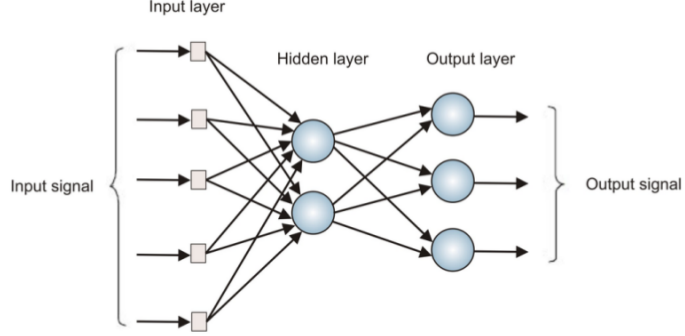
\includegraphics[width=0.8\textwidth]{nn.png}
\caption{\label{fig:nn}Structure of a Multi-layer Perceptron \cite{nn}.}
\end{figure}

Multilayer perceptron with single layer can solve a wide variety of problems. The weights can initially be assumed randomly and then the network can be trained by backpropagation \cite{bp}. The implementation given in \textit{scikitlearn} was used and the hyper-parameter values are given in Table~\ref{tab:nn1}. 

\begin{table}
\centering
\begin{tabular}{l|r}
hyper-parameter & values \\\hline
Train-Test split & 90:10 \\
Hidden-layer dimensions & 500, 100 \\
Activation Function & Relu \\
Optimizer & Adam \\
Regularization Coefficient & 0.0001 \\
Batch Size & 200 \\
Learning Rate & 0.001 (constant) \\
Maximum Iterations & 200 \\
Tolerance & 1e-4
\end{tabular}
\caption{\label{tab:nn1}Hyper-parameters for MLP setup.}
\end{table}

\subsection{Support Vector Regression}
Support Vector Machine can be applied not only to the classification problems but also to the regression problems. Similar to classification, the basic aim is to optimize the generalization bounds for regression \cite{svr}. It uses an epsilon intensive loss function which ignores errors that are situated within the certain distance of the true value. Figure~\ref{fig:sv} below shows an example of one-dimensional linear regression function with epsilon intensive band. The variables measure the cost of the errors on the training points. The error is zero for all points inside the epsilon band. SV algorithm can be made nonlinear by simply pre-processing the training patterns with kernel functions. In the nonlinear setting, the optimization problem corresponds to finding the flattest function in feature space, not in input space. The implementation given in \textit{scikitlearn} was used and the hyper-parameter values are given in Table~\ref{tab:svr1}.

\begin{figure}
\centering
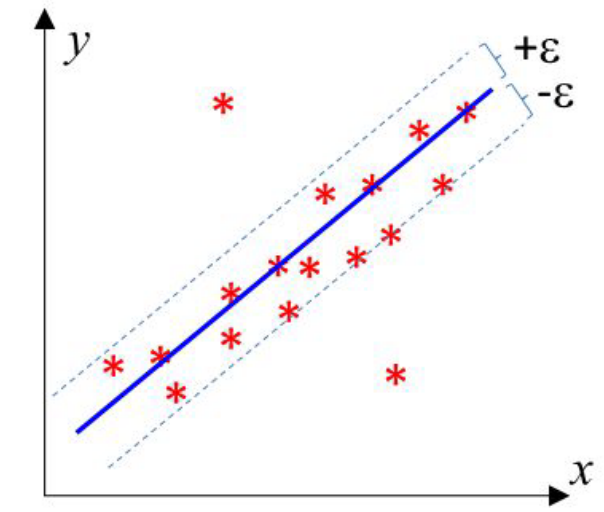
\includegraphics[width=0.5\textwidth]{sv.png}
\caption{\label{fig:sv}Linear regression function with epsilon insensitive band \cite{svr}.}
\end{figure} 

\begin{table}
\centering
\begin{tabular}{l|r}
hyper-parameter & values \\\hline
Train-Test split & 90:10 \\
C & 1.0 \\
Epsilon & 0.1 \\
Kernel & RBF \\
Tolerance & 1e-3
\end{tabular}
\caption{\label{tab:svr1}Hyper-parameters for SVR setup.}
\end{table}

\section{Evaluation and Analysis}

\subsection{Datasets}
Two TEDx videos were used of lengths 624 seconds and 719 seconds. Then acoustic feature datasets obtained were of dimensions 6373x620 and 6373x714. Feature selection reduced the dataset size to \textit{n}x620 and \textit{n}x714 where \textit{n} was a hyper-parameter. The eyeblink data had dimensions 620x1 and 714x1. 

\subsection{Evaluation Metric}
The $R^2$ score was used as a performance metric for the learning algorithms used in the last experiment. The coefficient $R^2$ is defined as: 
$$R^2 = (1 - \frac{u}{v})$$

, where $u$ is the residual sum of squares and $v$ is the total sum of squares. The best possible score is 1.0 and it can be negative (because the model can be arbitrarily worse). A constant model that always predicts the expected value of target, disregarding the input features, would get a $R^2$ score of 0.0.

\subsection{Results}
The $R^2$ results for both the MLP and SVR setups were obtained in the first four experiments mentioned below. Four different experiments were conducted with the feature selection and learning methods. In the fifth experiment, the relevant acoustic features were determined. Since only correlation analysis gave good results, relevant features were determined for this feature selection.

\subsubsection{Full Audience and Feature Selection with Eigen-analysis}

The follwing $R^2$ results were obtained for given reduced acoustic dataset sizes. Table~\ref{tab:carol1} gives results for Carol TEDx video and Table~\ref{tab:simon1} for Simon TEDx video. Figure~\ref{fig:f1} shows the plot for the best result obtained here.

\begin{table}
\centering
\begin{tabular}{ |p{3cm}||p{3cm}|p{3cm}|p{3cm}|  }
 \hline
 \multicolumn{3}{|c|}{$R^2 scores$} \\
 \hline
 Dataset Size &MLP &SVR\\
 \hline
 10 & -0.13 &-0.006\\
 20 & 0.12 & 0.08\\
 50 & -0.09 & 0.20\\
 100 & -0.90 & 0.16\\
 200 & -1.52 & 0.24\\
 \hline
\end{tabular}
\caption{\label{tab:carol1}Results for Carol Video.}
\end{table}

\begin{table}
\centering
\begin{tabular}{ |p{3cm}||p{3cm}|p{3cm}|p{3cm}|  }
 \hline
 \multicolumn{3}{|c|}{$R^2 scores$} \\
 \hline
 Dataset Size &MLP &SVR\\
 \hline
 10 & -0.18 &-0.12\\
 20 & 0.29 & 0.16\\
 50 & 0.03 & 0.13\\
 100 & -0.30 & 0.19\\
 200 & -0.28 & 0.25\\
 \hline
\end{tabular}
\caption{\label{tab:simon1}Results for Simon Video.}
\end{table}

\begin{figure}
\centering
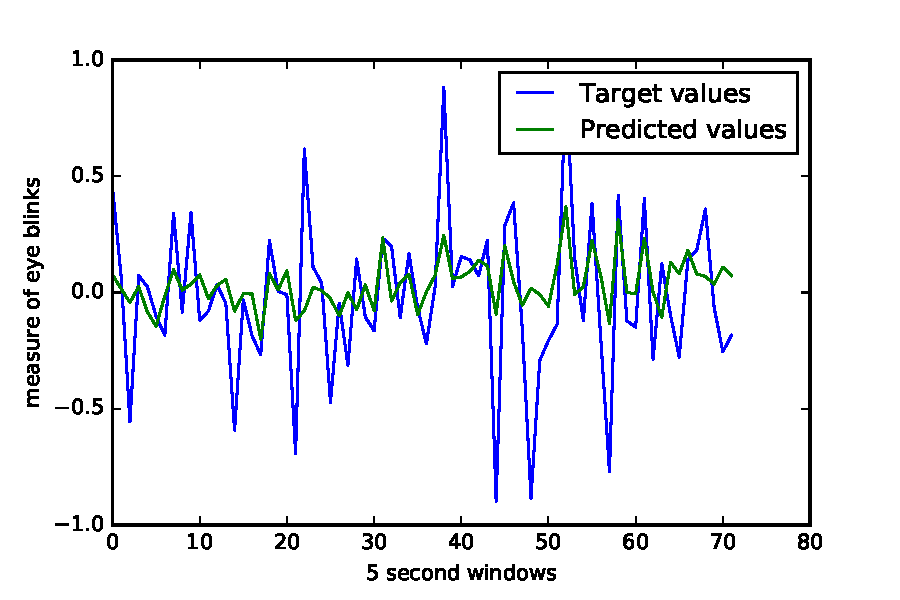
\includegraphics[width=0.4\textwidth]{f1.pdf}
\caption{\label{fig:f1}Plot for Simon Video with SVR and size 200.}
\end{figure} 

\subsubsection{Full Audience and Feature Selection with Correlation-analysis}

The follwing $R^2$ results were obtained for given reduced acoustic dataset sizes. Table~\ref{tab:carol2} gives results for Carol TEDx video and Table~\ref{tab:simon2} for Simon TEDx video. Figure~\ref{fig:f2} shows the plot for the best result obtained here.

\begin{table}
\centering
\begin{tabular}{ |p{3cm}||p{3cm}|p{3cm}|p{3cm}|  }
 \hline
 \multicolumn{3}{|c|}{$R^2 scores$} \\
 \hline
 Dataset Size &MLP &SVR\\
 \hline
 10 & 0.23 & 0.11\\
 20 & 0.47 & 0.44\\
 50 & 0.38 & 0.43\\
 100 & 0.26 & 0.48\\
 200 & 0.19 & 0.44\\
 \hline
\end{tabular}
\caption{\label{tab:carol2}Results for Carol Video.}
\end{table}

\begin{table}
\centering
\begin{tabular}{ |p{3cm}||p{3cm}|p{3cm}|p{3cm}|  }
 \hline
 \multicolumn{3}{|c|}{$R^2 scores$} \\
 \hline
 Dataset Size &MLP &SVR\\
 \hline
 10 & 0.31 & 0.21\\
 20 & 0.48 & 0.40\\
 50 & 0.54 & 0.45\\
 100 & 0.48 & 0.52\\
 200 & 0.45 & 0.55\\
 \hline
\end{tabular}
\caption{\label{tab:simon2}Results for Simon Video.}
\end{table}

\begin{figure}
\centering
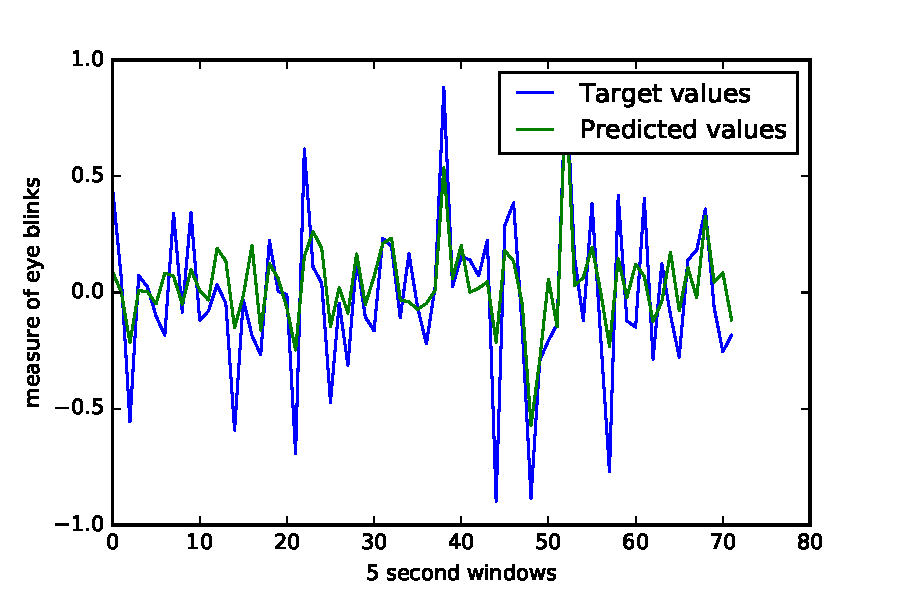
\includegraphics[width=0.4\textwidth]{f2.pdf}
\caption{\label{fig:f2}Plot for Simon Video with SVR and size 200.}
\end{figure} 

\subsubsection{Reduced Audience and Feature Selection with Eigen-analysis}

The follwing $R^2$ results were obtained for given reduced acoustic dataset sizes. Table~\ref{tab:carol3} gives results for Carol TEDx video and Table~\ref{tab:simon3} for Simon TEDx video. Figure~\ref{fig:f3} shows the plot for the best result obtained here.

\begin{table}
\centering
\begin{tabular}{ |p{3cm}||p{3cm}|p{3cm}|p{3cm}|  }
 \hline
 \multicolumn{3}{|c|}{$R^2 scores$} \\
 \hline
 Dataset Size &MLP &SVR\\
 \hline
 10 & -0.52 & 0.09\\
 20 & -0.03 & 0.28\\
 50 & -0.008 & 0.31\\
 100 & 0.03 & 0.32\\
 200 & -0.68 & 0.29\\
 \hline
\end{tabular}
\caption{\label{tab:carol3}Results for Carol Video.}
\end{table}

\begin{table}
\centering
\begin{tabular}{ |p{3cm}||p{3cm}|p{3cm}|p{3cm}|  }
 \hline
 \multicolumn{3}{|c|}{$R^2 scores$} \\
 \hline
 Dataset Size &MLP &SVR\\
 \hline
 10 & -0.32 & -0.114\\
 20 & 0.12 & 0.095\\
 50 & 0.26 & 0.14\\
 100 & 0.20 & 0.17\\
 200 & -0.17 & 0.16\\
 \hline
\end{tabular}
\caption{\label{tab:simon3}Results for Simon Video.}
\end{table}

\begin{figure}
\centering
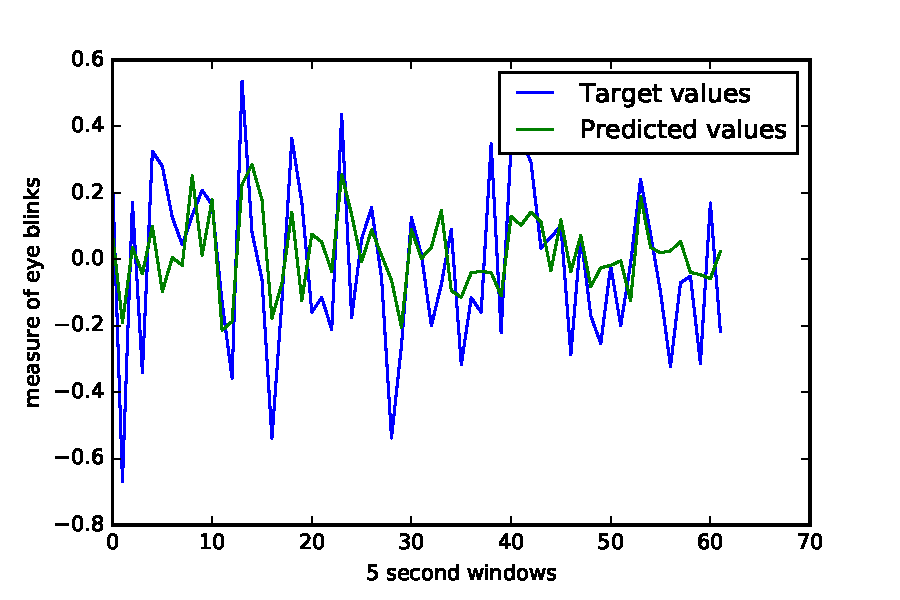
\includegraphics[width=0.4\textwidth]{f3.pdf}
\caption{\label{fig:f3}Plot for Carol Video with SVR and size 100.}
\end{figure} 

\subsubsection{Reduced Audience and Feature Selection with Correlation-analysis}

The follwing $R^2$ results were obtained for given reduced acoustic dataset sizes. Table~\ref{tab:carol4} gives results for Carol TEDx video and Table~\ref{tab:simon4} for Simon TEDx video. Figure~\ref{fig:f4} shows the plot for the best result obtained here.

\begin{table}
\centering
\begin{tabular}{ |p{3cm}||p{3cm}|p{3cm}|p{3cm}|  }
 \hline
 \multicolumn{3}{|c|}{$R^2 scores$} \\
 \hline
 Dataset Size &MLP &SVR\\
 \hline
 10 & 0.004 & 0.14\\
 20 & 0.34 & 0.40\\
 50 & 0.36 & 0.48\\
 100 & 0.39 & 0.51\\
 200 & 0.20 & 0.53\\
 \hline
\end{tabular}
\caption{\label{tab:carol4}Results for Carol Video.}
\end{table}

\begin{table}
\centering
\begin{tabular}{ |p{3cm}||p{3cm}|p{3cm}|p{3cm}|  }
 \hline
 \multicolumn{3}{|c|}{$R^2 scores$} \\
 \hline
 Dataset Size &MLP &SVR\\
 \hline
 10 & 0.27 & 0.34\\
 20 & 0.51 & 0.43\\
 50 & 0.47 & 0.52\\
 100 & 0.48 & 0.53\\
 200 & 0.51 & 0.57\\
 \hline
\end{tabular}
\caption{\label{tab:simon4}Results for Simon Video.}
\end{table}

\begin{figure}
\centering
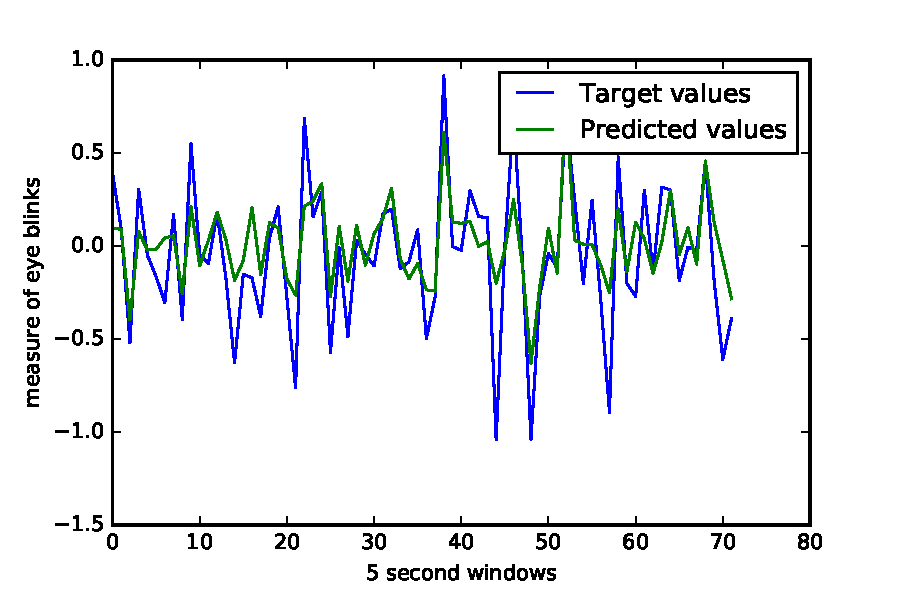
\includegraphics[width=0.4\textwidth]{f4.pdf}
\caption{\label{fig:f4}Plot for Simon Video with SVR and size 200.}
\end{figure} 

\subsubsection{Relevant Features with respect to Attention}
Only the correlation-analysis gave good results. Therefore the relevant features obtained through this feature selection were determined for both the full audience case and reduced one.

Top 10 features for Carol video with Full Audience:
\begin{itemize}
\item \verb|audspec_lengthL1norm_sma_stddev|:standard deviation of magnitude of the L1 norm of auditory spectrum and it was smoothed using an averaging filter with window length 3.
\item \verb|audSpec_Rfilt_sma[0]_range|:Rfilt means Relative Spectral Transform (RASTA)-style filtered. This means range of 0th Rfilt of auditory spectrum and it was smoothed using an averaging filter with window length 3.
\item \verb|audSpec_Rfilt_sma[19]_percentile1.0|:Rfilt means Relative Spectral Transform (RASTA)-style filtered. Percentile1.0 is the outlier-robust minimum value of the contour, represented by the 1 percentile. This means percentile1.0 of 19th Rfilt of auditory spectrum and it was smoothed using an averaging filter with window length 3.
\item \verb|audSpec_Rfilt_sma[24]_range|:Rfilt means Relative Spectral Transform (RASTA)-style filtered. This means range of 24th Rfilt of auditory spectrum and it was smoothed using an averaging filter with window length 3.
\item \verb|audSpec_Rfilt_sma[25]_percentile1.0|:Rfilt means Relative Spectral Transform (RASTA)-style filtered. Percentile1.0 is the outlier-robust minimum value of the contour, represented by the 1 percentile. This means percentile1.0 of 25th Rfilt of auditory spectrum and it was smoothed using an averaging filter with window length 3.
\item \verb|pcm_fftMag_spectralRollOff75.0_sma_leftctime|: The 75 ∗ 100 percent spectral roll-off point is determined as the frequency below which 75 ∗ 100 percent of the total signal energy fall. This means time during which the spectralRollOff75.0 of fast Fourier transformed pulse-code modulation has left curvature and it was smoothed using an averaging filter with window length 3.
\item \verb|mfcc_sma[2]_range|:range of 2nd mel-frequency cepstral coefficient and it was smoothed using an averaging filter with window length 3.
\item \verb|mfcc_sma[4]_percentile1.0|:Percentile1.0 is the outlier-robust minimum value of the contour, represented by the 1 percentile. This means percentile1.0 of 4th mel-frequency cepstral coefficient and it was smoothed using an averaging filter with window length 3.
\item \verb|mfcc_sma[8]_percentile99.0|:Percentile99.0 is the outlier-robust maximum value of the contour, represented by the 99 percentile. This means percentile99.0 of 8th mel-frequency cepstral coefficient and it was smoothed using an averaging filter with window length 3.
\item \verb|mfcc_sma_de[4]_range|:range of 4th mel-frequency cepstral coefficient and it was smoothed using an averaging filter with window length 3.
\end{itemize}

Top 10 features for Simon video with Full Audience:
\begin{itemize}
\item \verb|pcm_zcr_sma_percentile99.0|:Percentile99.0 is the outlier-robust maximum value of the contour, represented by the 99 percentile. This means percentile99.0 of zero-crossing rate of time signal and it was smoothed using an averaging filter with window length 3.
\item \verb|audspec_lengthL1norm_sma_de_range|:range of magnitude of the L1 norm of auditory spectrum and it was smoothed using an averaging filter with window length 3.
\item \verb|audSpec_Rfilt_sma[9]_range|:Rfilt means Relative Spectral Transform (RASTA)-style filtered. This means range of 9th Rfilt of auditory spectrum and it was smoothed using an averaging filter with window length 3.
\item \verb|audSpec_Rfilt_sma[15]_range|:Rfilt means Relative Spectral Transform (RASTA)-style filtered. This means range of 15th Rfilt of auditory spectrum and it was smoothed using an averaging filter with window length 3.
\item \verb|audSpec_Rfilt_sma[16]_pctlrange0-1|:Rfilt means Relative Spectral Transform (RASTA)-style filtered. This means 0-1 inter-percentile range of 16th Rfilt of auditory spectrum and it was smoothed using an averaging filter with window length 3.
\item \verb|pcm_fftMag_spectralRollOff25.0_sma_range|: The 25 ∗ 100 percent spectral roll-off point is determined as the frequency below which 25 ∗ 100 percent of the total signal energy fall. This means range of spectralRollOff25.0 of fast Fourier transformed pulse-code modulation and it was smoothed using an averaging filter with window length 3.
\item \verb|pcm_fftMag_spectralHarmonicity_sma_range|:A Harmonicity object represents the degree of acoustic periodicity, also called Harmonics-to-Noise Ratio (HNR). This means range of spectral harmonicity of fast Fourier transformed pulse-code modulation and it was smoothed using an averaging filter with window length 3.
\item \verb|audSpec_Rfilt_sma_de[8]_range|:Rfilt means Relative Spectral Transform (RASTA)-style filtered. This means range of 8th Rfilt of auditory spectrum and it was smoothed using an averaging filter with window length 3.
\item \verb|pcm_fftMag_spectralSlope_sma_peakRangeAbs|:absolute value of range of all values for spectral slope of fast Fourier transformed pulse-code modulation and it was smoothed using an averaging filter with window length 3.
\item \verb|audspec_lengthL1norm_sma_de_peakRangeAbs|:absolute value of range of all values for magnitude of the L1 norm of auditory spectrum and it was smoothed using an averaging filter with window length 3.
\end{itemize}

Top 10 features for Carol video with Reduced Audience:
\begin{itemize}
\item \verb|audspec_lengthL1norm_sma_quartile2|:$50th$ percentile of magnitude of the L1 norm of auditory spectrum and it was smoothed using an averaging filter with window length 3.
\item \verb|pcm_RMSenergy_sma_percentile99.0|:Percentile99.0 is the outlier-robust maximum value of the contour, represented by the 99 percentile. This means percentile99.0 of root-mean-square signal frame energy and it was smoothed using an averaging filter with window length 3.
\item \verb|pcm_RMSenergy_sma_pctlrange0-1|:This means 0-1 inter-percentile range of root-mean-square signal frame energy and it was smoothed using an averaging filter with window length 3.
\item \verb|audSpec_Rfilt_sma[20]_percentile1.0|:Rfilt means Relative Spectral Transform (RASTA)-style filtered. Percentile1.0 is the outlier-robust minimum value of the contour, represented by the 1 percentile. This means percentile1.0 of 20th Rfilt of auditory spectrum and it was smoothed using an averaging filter with window length 3.
\item \verb|mfcc_sma[1]_percentile99.0|:Percentile99.0 is the outlier-robust maximum value of the contour, represented by the 99 percentile. This means percentile99.0 of 1st mel-frequency cepstral coefficient and it was smoothed using an averaging filter with window length 3.
\item \verb|audSpec_Rfilt_sma_de[23]_percentile99.0|:Rfilt means Relative Spectral Transform (RASTA)-style filtered. Percentile99.0 is the outlier-robust maximum value of the contour, represented by the 99 percentile. This means percentile99.0 of 25th Rfilt of auditory spectrum and it was smoothed using an averaging filter with window length 3.
\item \verb|audSpec_Rfilt_sma[6]_meanRisingSlope|:meanRisingSlope is the mean of rising slopes, i.e. the slopes connecting a valley with the following peak. Rfilt means Relative Spectral Transform (RASTA)-style filtered. This means meanRisingSlope of 6th Rfilt of auditory spectrum and it was smoothed using an averaging filter with window length 3.
\item \verb|pcm_fftMag_spectralRollOff50.0_sma_minRangeRel|:The 50 ∗ 100 percent spectral roll-off point is determined as the frequency below which 50 ∗ 100 percent of the total signal energy fall. This means minimum value of relative range of spectralRollOff50.0 of fast Fourier transformed pulse-code modulation and it was smoothed using an averaging filter with window length 3.
\item \verb|audSpec_Rfilt_sma_de[21]_peakMeanAbs|:Rfilt means Relative Spectral Transform (RASTA)-style filtered. This means absolute value of mean of all values for 21th Rfilt of auditory spectrum and it was smoothed using an averaging filter with window length 3.
\item \verb|audSpec_Rfilt_sma_de[21]_peakMeanMeanDist|:Rfilt means Relative Spectral Transform (RASTA)-style filtered. This means mean of distance between peaks for 21th Rfilt of auditory spectrum and it was smoothed using an averaging filter with window length 3.
\end{itemize}

Top 10 features for Simon video with Reduced Audience:
\begin{itemize}
\item \verb|audSpec_Rfilt_sma[13]_range|:Rfilt means Relative Spectral Transform (RASTA)-style filtered. This means range of 13th Rfilt of auditory spectrum and it was smoothed using an averaging filter with window length 3.
\item \verb|audSpec_Rfilt_sma[23]_range|:Rfilt means Relative Spectral Transform (RASTA)-style filtered. This means range of 23th Rfilt of auditory spectrum and it was smoothed using an averaging filter with window length 3.
\item \verb|pcm_fftMag_spectralRollOff25.0_sma_percentile99.0|:Percentile99.0 is the outlier-robust maximum value of the contour, represented by the 99 percentile. The 25 ∗ 100 percent spectral roll-off point is determined as the frequency below which 25 ∗ 100 percent of the total signal energy fall. This means percentile99.0 of spectralRollOff25.0 of fast Fourier transformed pulse-code modulation and it was smoothed using an averaging filter with window length 3.
\item \verb|pcm_fftMag_spectralFlux_sma_range|:range of spectral flux of fast Fourier transformed pulse-code modulation and it was smoothed using an averaging filter with window length 3.
\item \verb|pcm_fftMag_spectralSkewness_sma_range|:Spectral skewness is a measure of the asymmetry of the spectral distribution around its centroid. This means range of spectral skewness of fast Fourier transformed pulse-code modulation and it was smoothed using an averaging filter with window length 3.
\item \verb|pcm_fftMag_psySharpness_sma_percentile1.0|:psySharpness is related to how much a sound’s spectrum is in the high end. Percentile1.0 is the outlier-robust minimum value of the contour, represented by the 1 percentile. This means percentile1.0 of psySharpness of fast Fourier transformed pulse-code modulation and it was smoothed using an averaging filter with window length 3.
\item \verb|mfcc_sma[6]_percentile1.0|:Percentile1.0 is the outlier-robust minimum value of the contour, represented by the 1 percentile. This means percentile1.0 of 6th mel-frequency cepstral coefficient and it was smoothed using an averaging filter with window length 3.
\item \verb|audSpec_Rfilt_sma_de[20]_range|:Rfilt means Relative Spectral Transform (RASTA)-style filtered. This means range of 20th Rfilt of auditory spectrum and it was smoothed using an averaging filter with window length 3.
\item \verb|pcm_fftMag_spectralFlux_sma_de_range|:delta of range of spectral flux of fast Fourier transformed pulse-code modulation and it was smoothed using an averaging filter with window length 3.
\item \verb|audSpec_Rfilt_sma_de[5]_stddevRisingSlope|:stddevRisingSlope is the standard deviation of rising slopes, i.e. the slopes connecting a valley with the following peak. Rfilt means Relative Spectral Transform (RASTA)-style filtered. This means stddevRisingSlope of 5th Rfilt of auditory spectrum and it was smoothed using an averaging filter with window length 3.
\end{itemize}

\section{Conclusion}

Best results were obtained using the correlation based feature selection for both the full audience and reduced audience case. For the full audience experiment, the best results were obtained for Simon video with SVR and correlation based feature selection of 200 features. Again for reduced dataset experiment, the best results were obtained for Simon video with SVR and correlation based feature selection of 200 features. The SVR learning method consistently out-performed the MLP method. 

The relevant audio features were also obtained for both the experiments. Future work can include further interpretation of the relevant features obtained. Also some other audio feature extraction methods can be explored. 


\begin{thebibliography}{9}
\bibitem{political} 
Zhang, John R., et al.
\textit{Correlating Speaker Gestures in Political Debates with Audience Engagement Measured via EEG}. 
Proceedings of the ACM International Conference on Multimedia. ACM, 2014.

\bibitem{opensmile} 
Eyben, Florian, Martin Wllmer, and Bjrn Schuller.
\textit{Opensmile: the munich versatile and fast open-source audio feature extractor}. 
Proceedings of the international conference on Multimedia. ACM, 2010.

\bibitem{compare} 
Schuller, Bjrn, et al.
\textit{The INTERSPEECH 2013 computational paralinguistics challenge: social signals, conflict, emotion, autism}. 
(2013).

\bibitem{audio} 
Eyben, Florian, et al.
\textit{The acoustics of eye contact: detecting visual attention from conversational audio cues}. 
Proceedings of the 6th workshop on Eye gaze in intelligent human machine interaction: gaze in multimodal interaction. ACM, 2013.

\bibitem{ffmpeg} 
Bellard, Fabrice, and M. Niedermayer.
\textit{FFmpeg}. 
http://ffmpeg.org (2012).

\bibitem{scikit} 
Pedregosa et al.
\textit{Scikit-learn: Machine Learning in Python}. 
JMLR 12, pp. 2825-2830, 2011.

\bibitem{nn} 
M.W.Gardener, S.R. Dorling.
\textit{ARTIFICIAL Neural Networks(The Multilayer perceptron)- A review of the applications in Atmospheric Sciences}. 
June 1998.

\bibitem{bp} 
Christopher Bishop.
\textit{Pattern Recognition and Machine Learning}. 
book, (2007).

\bibitem{svr} 
Alex J. Samola, Bernard S.
\textit{A tutorial on Support Vector Regression}. 
NeuroCOLT2 Technical Report NCR2, October 1998.

\end{thebibliography}

%\bibliography{references}

\end{document} to your LaTeX file where you want your
% title page.
%
%%%%%%%%%%%%%%%%%%%%%%%%%%%%%%%%%%%%%%%%%
%\title{Title page with logo}
%----------------------------------------------------------------------------------------
%	PACKAGES AND OTHER DOCUMENT CONFIGURATIONS
%----------------------------------------------------------------------------------------

\documentclass[12pt]{article}
\usepackage[english]{babel}
\usepackage[utf8x]{inputenc}
\usepackage{amsmath}
\usepackage{graphicx}
\usepackage[colorinlistoftodos]{todonotes}

\begin{document}

\begin{titlepage}

\newcommand{\HRule}{\rule{\linewidth}{0.5mm}} % Defines a new command for the horizontal lines, change thickness here

\center % Center everything on the page
 
%----------------------------------------------------------------------------------------
%	HEADING SECTIONS
%----------------------------------------------------------------------------------------

\textsc{\LARGE Columbia University}\\[1.5cm] % Name of your university/college
\textsc{\Large Project Report}\\[0.5cm] % Major heading such as course name
\textsc{\large COMS 6901}\\[0.5cm] % Minor heading such as course title

%----------------------------------------------------------------------------------------
%	TITLE SECTION
%----------------------------------------------------------------------------------------

\HRule \\[0.4cm]
{ \Large \bfseries Correlation of acoustic features of speakers with Audience Engagement}\\[0.5cm] % Title of your document
\HRule \\[0.5cm]
 
%----------------------------------------------------------------------------------------
%	AUTHOR SECTION
%----------------------------------------------------------------------------------------

\begin{minipage}{0.4\textwidth}
\begin{flushleft} \large
\emph{Author:}\\
Animesh Sharma % Your name
\end{flushleft}
\end{minipage}
~
\begin{minipage}{0.4\textwidth}
\begin{flushright} \large
\emph{Supervisor:} \\
Dr. John Kender % Supervisor's Name
\end{flushright}
\end{minipage}\\[2cm]

% If you don't want a supervisor, uncomment the two lines below and remove the section above
%\Large \emph{Author:}\\
%John \textsc{Smith}\\[3cm] % Your name

%----------------------------------------------------------------------------------------
%	DATE SECTION
%----------------------------------------------------------------------------------------

{\large \today}\\[1cm] % Date, change the \today to a set date if you want to be precise

%----------------------------------------------------------------------------------------
%	LOGO SECTION
%----------------------------------------------------------------------------------------


\includegraphics{CU_logo.jpg}\\[0.5cm] % Include a department/university logo - this will require the graphicx package
 
%----------------------------------------------------------------------------------------

\vfill % Fill the rest of the page with whitespace

\end{titlepage}

\begin{abstract}
In this work, we investigate the extent to which the acoustic features of speakers are correlated to the audience engagement. The number of eyeblinks in a particular time period was taken as a measure of engagement of audience and the acoustic feature set of size 6373 was obtained for two different TEDx videos- Simon and Carol, with the help of OpenSmile software. Then eigen-analysis and mutual info regression based correlation analysis were used for feature selection in case of audio feature set. In order to determine the extent to which the acoustic features are correlated with the attention signal, two learning algorithms- Multi-layer Perceptron (MLP) and Support Vector Regression (SVR), were used to predict the attention signal with the acoustic feature set being used as input to the network. The best $R^2$ score of 0.55 was obtained for the correlation based analysis of Simon video with Support Vector Regression and acoustic feature set of size 200. Then the anomalies in audience, which were previously being handled through Z-score, were removed and all the experiments were performed again. This time the best result was 0.57 for Simon video with correlation based analysis and Support Vector Regression. The audio features most correlated with eyeblink data were also listed for both cases with feature selection based on correlation analysis.
\end{abstract}

\clearpage

\tableofcontents

\clearpage

\section{Introduction}

This project is based on the work done by Zhang et al. \cite{political}. in which the authors propose that certain speaker gestures can convey important information regarding audience engagement. Two TEDx videos, labeled Simon and Carol, were used for this project and it was studied whether certain acoustic features have more influence on the audience engagement. This work is useful in determining whether audience engagement can be improved with the help of the observed acoustic features. The acoustic features most correlated with the audience engagement can help instructors and speakers in further engaging their audience. The eyeblink data was used as a measure of the audience engagement based on the premise that the subject tends to pay more attention when the number of eyeblinks are less for that time period. There were 28 subjects for both the videos and the number of eyeblinks for a 5 second window were obtained for the audience as a whole by taking the mean for that time period. The acoustic feature dataset of size 6373 was obtained using OpenSmile \cite{opensmile}. software and this dataset was then used as input to the learning algorithms. This acoustic feature set, known as ComParE feature set \cite{compare}, was given by Eybet et al \cite{audio} and they are functionals of acoustic low level descriptors (LLDs). Then feature selection was done for the audio feature set so as to evaluate the performance of the learning algorithms only on the relevant features and to filter out the noise. The learning algorithms were used to determine whether the attention signal can be predicted with acoustic signal as input. The performance of the learning algorithm give a sense of the importance of audio features in determing the audience engagement. Furthermore, the important audio features determined by correlating them with attention signal can also be listed so that it can be known which audio features out of the feature set of size 6373 influence the attention signal most. Predicting the attention signal is a regression problem and two different learning algorithms were used for the same. One important issue with this task was handling the anomalies present in the eyeblink dataset of audience. Some of the eyeblink recordings of the subjects were corrupted in the sense that there were two many eyeblinks in certain 5 second windows. These anomalies were handled by taking Z-scores of the recordings in first case and afterwards removing them in the second. All the steps were repeated for both the cases.

\section{Problem Formulation}

Two different datasets- eyeblink dataset and acoustic feature dataset, were prepared for this work and then subsequent analysis was done for determining how much one is correlated with the other.The whole project pipeline has 5 subsections and these were executed in-order to obtain the final result. The following contributions were made in this work:
\begin{enumerate}
\item The eyeblink data was cleaned and pre-processed to get an attention signal for the audience. The experiments were conducted first for all the 28 subjects in audience and then the anomalies were removed and the experiments were repeated for 17 subjects. The outlier subjects were removed on the criteria that for these subjects, the number of eyeblinks in a 5 second window was too high for a human being.
\item The acoustic feature dataset was prepared for the two TEDx videos for 5 second windows using OpenSmile software. The audio was stripped off from the video file and 5 second windows were obtained using ffmpeg wrapper \cite{ffmpeg}. 
\item The acoustic feature set of size 6373 was reduced to sizes 10, 20, 50, 100 and 200 using eigenanalysis and mutual information based correlation analysis. The scikit-learn library in Python \cite{scikit} was used for this feature selection. The reduced feature set in eigenanalysis was further preprocessed using Z-score method.
\item Then it was determined whether its possible to predict the attention of the audience with reduced acoustic feature set. Two different learning algorithms were used - Neural Networks and Support Vector Regression. The scikit-learn was again used here and the network settings for both the methods are defined in subsequent sections.
\item The different acoustic features obtained for both the full audience and the reduced audience were also listed and the meaning of these features was obtained so that it can be determined which characteristics of a person's speech are helpful in capturing attention of the audience.  
\end{enumerate}

\section{Proposed Method}
\label{sec:methods}

The following subsections define the different submodules executed for obtaining the final result given in this work. 

\subsection{Eyeblink data cleaning and preprocessing}

The raw data was in xls format and there were many redundant columns in it. The format was converted to csv. Multiple scripts in python were written for different preprocessing tasks. Only the follwing columns were retained- \verb|CURRENT_FIX_LABEL| column which gives the fixation timestamp and the \verb|NEXT_SAC_CONTAINS_BLINK| column which gives boolean values as to whether this section contains eyeblink or not. The data of the fixation column was converted to integer values and then the number of eyeblinks in a 5 second window was obtained. The Z-score values were obtained so as to normalize the eyeblink data with respect to each subject individually. Finally the mean of the eyeblink data for the audience was taken for each 5 second window.

\subsection{Handling Outliers in Eyeblink dataset}

For the first experiment, just the Z-score values were obtained for all the subjects. It was done so as to diffuse the effect of the outliers. There were 28 subjects for both the Simon and Carol video.

For the second experiment, the anomalies were removed for both the Simon and Carol videos. For the Carol video, the following subjects were removed with the given reasons:
\begin{itemize}
\item \verb|jc1_carol|: consistent eyeblinks of 6 or 5
\item \verb|jhh1_carol|, \verb|msb1_carol|: consistently high eyeblinks of 10
\item \verb|jy1_carol|, \verb|pp1_carol|, \verb|rn1_carol|: no eyeblinks at all (0 or 1)
\item \verb|pc1_carol|: lots of 10 at the end of the video
\item \verb|sa1_carol|, \verb|sd2_carol|, \verb|sw1_carol|, \verb|ys1_carol|: consistently high eyeblinks
\end{itemize}
\clearpage
For the Simon video, the following subjects were removed with the given reasons:
\begin{itemize}
\item \verb|jg1_simon|, \verb|pp1_simon|, \verb|rn1_simon|, \verb|jy1_simon|: no eyeblinks at all (0 or 1)
\item \verb|sa1_simon|, \verb|jc1_simon|, \verb|sd2_simon|, \verb|klt1_simon|, \verb|azz1_simon|, \verb|ys1_simon|, \verb|jhh1_simon|: consistently high eyeblinks
\end{itemize}

\subsection{Acoustic Feature Set}
The audio was extracted from the video files in \textit{mp3} format and then it was converted to \textit{wav} format using ffmpeg wrapper. Then a script in \textit{Ruby} was written to obtain 5 second windows for both the TEDx files and the offset was taken as 1 second here. Finally the ComParE audio feature set of size 6373 was obtained using OpenSmile and the output format was \textit{csv}.

The length of the Carol video was 624 seconds and therefore 620 fragments were obtained for this file. Similarly, 714 fragments were obtained for the Simon video with length 718 seconds.

\subsection{Feature Selection for Acoustic Feature Set}
Two different methods were used for reducing the size of the ComParE dataset obtained using OpenSmile. First the size was reduced using Eigenanalysis. The \textit{sklearn} package present in \textit{Python} was used here to reduce the dataset size to 10, 20, 50, 100 and 200. Then the values were normalized using Z-score method.

For the second method, correlation with the eyeblink data was used to select only \textit{n} features out of the 6373 available so that the selected features have highest correlation values. The method used here to calculate the correlation values was \textit{mutual info regression} present in \textit{sklearn} package. The reduced dataset sizes were again 10, 20, 50, 100 and 200 and the predefined method \textit{SelectKBest} available in \textit{scikitlearn} was used.

\subsection{Neural Networks}
A Multi-layer perceptron is a network of simple neurons called Perceptron. Each neuron computes the output which is some linear or usually a non-linear function of the linear combination of the input and the weights including the bias. A simple neuron has mapping limitations and thus a number or layers with a large number of neurons are used. The input neuron layer represents each instance which is fed to the hidden layer. The hidden layer computes the output depending on the input it receives, the corresponding weights and the activation function which is then fed to the output layer \cite{nn}. Thus the input signal propagates the network layer by layer. The number of the layers depends on the structure of the network. Figure~\ref{fig:nn} shows the structure of a multi-layer perceptron.

\begin{figure}
\centering
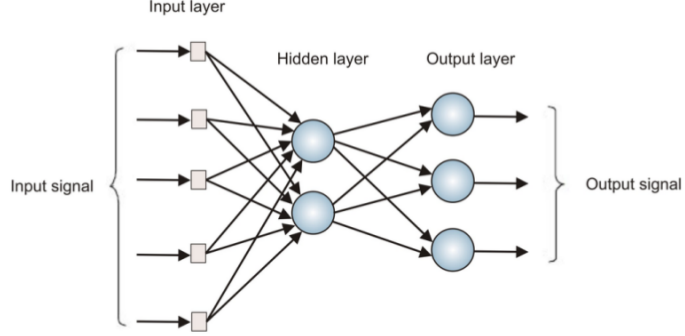
\includegraphics[width=0.8\textwidth]{nn.png}
\caption{\label{fig:nn}Structure of a Multi-layer Perceptron \cite{nn}.}
\end{figure}

Multilayer perceptron with single layer can solve a wide variety of problems. The weights can initially be assumed randomly and then the network can be trained by backpropagation \cite{bp}. The implementation given in \textit{scikitlearn} was used and the hyper-parameter values are given in Table~\ref{tab:nn1}. 

\begin{table}
\centering
\begin{tabular}{l|r}
hyper-parameter & values \\\hline
Train-Test split & 90:10 \\
Hidden-layer dimensions & 500, 100 \\
Activation Function & Relu \\
Optimizer & Adam \\
Regularization Coefficient & 0.0001 \\
Batch Size & 200 \\
Learning Rate & 0.001 (constant) \\
Maximum Iterations & 200 \\
Tolerance & 1e-4
\end{tabular}
\caption{\label{tab:nn1}Hyper-parameters for MLP setup.}
\end{table}

\subsection{Support Vector Regression}
Support Vector Machine can be applied not only to the classification problems but also to the regression problems. Similar to classification, the basic aim is to optimize the generalization bounds for regression \cite{svr}. It uses an epsilon intensive loss function which ignores errors that are situated within the certain distance of the true value. Figure~\ref{fig:sv} below shows an example of one-dimensional linear regression function with epsilon intensive band. The variables measure the cost of the errors on the training points. The error is zero for all points inside the epsilon band. SV algorithm can be made nonlinear by simply pre-processing the training patterns with kernel functions. In the nonlinear setting, the optimization problem corresponds to finding the flattest function in feature space, not in input space. The implementation given in \textit{scikitlearn} was used and the hyper-parameter values are given in Table~\ref{tab:svr1}.

\begin{figure}
\centering
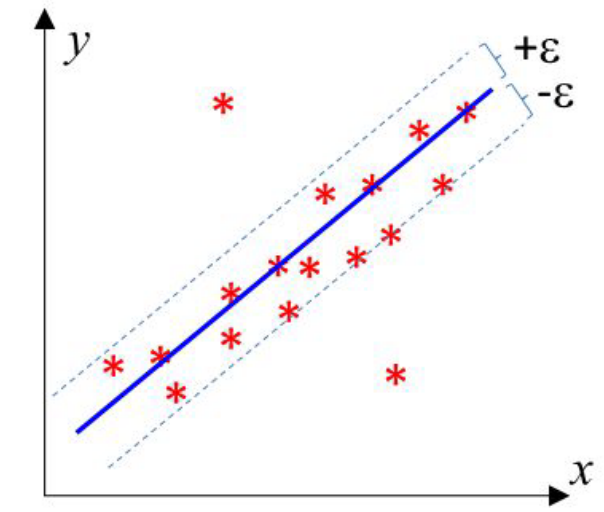
\includegraphics[width=0.5\textwidth]{sv.png}
\caption{\label{fig:sv}Linear regression function with epsilon insensitive band \cite{svr}.}
\end{figure} 

\begin{table}
\centering
\begin{tabular}{l|r}
hyper-parameter & values \\\hline
Train-Test split & 90:10 \\
C & 1.0 \\
Epsilon & 0.1 \\
Kernel & RBF \\
Tolerance & 1e-3
\end{tabular}
\caption{\label{tab:svr1}Hyper-parameters for SVR setup.}
\end{table}

\section{Evaluation and Analysis}

\subsection{Datasets}
Two TEDx videos were used of lengths 624 seconds and 719 seconds. Then acoustic feature datasets obtained were of dimensions 6373x620 and 6373x714. Feature selection reduced the dataset size to \textit{n}x620 and \textit{n}x714 where \textit{n} was a hyper-parameter. The eyeblink data had dimensions 620x1 and 714x1. 

\subsection{Evaluation Metric}
The $R^2$ score was used as a performance metric for the learning algorithms used in the last experiment. The coefficient $R^2$ is defined as: 
$$R^2 = (1 - \frac{u}{v})$$

, where $u$ is the residual sum of squares and $v$ is the total sum of squares. The best possible score is 1.0 and it can be negative (because the model can be arbitrarily worse). A constant model that always predicts the expected value of target, disregarding the input features, would get a $R^2$ score of 0.0.

\subsection{Results}
The $R^2$ results for both the MLP and SVR setups were obtained in the first four experiments mentioned below. Four different experiments were conducted with the feature selection and learning methods. In the fifth experiment, the relevant acoustic features were determined. Since only correlation analysis gave good results, relevant features were determined for this feature selection.

\subsubsection{Full Audience and Feature Selection with Eigen-analysis}

The follwing $R^2$ results were obtained for given reduced acoustic dataset sizes. Table~\ref{tab:carol1} gives results for Carol TEDx video and Table~\ref{tab:simon1} for Simon TEDx video. Figure~\ref{fig:f1} shows the plot for the best result obtained here.

\begin{table}
\centering
\begin{tabular}{ |p{3cm}||p{3cm}|p{3cm}|p{3cm}|  }
 \hline
 \multicolumn{3}{|c|}{$R^2 scores$} \\
 \hline
 Dataset Size &MLP &SVR\\
 \hline
 10 & -0.13 &-0.006\\
 20 & 0.12 & 0.08\\
 50 & -0.09 & 0.20\\
 100 & -0.90 & 0.16\\
 200 & -1.52 & 0.24\\
 \hline
\end{tabular}
\caption{\label{tab:carol1}Results for Carol Video.}
\end{table}

\begin{table}
\centering
\begin{tabular}{ |p{3cm}||p{3cm}|p{3cm}|p{3cm}|  }
 \hline
 \multicolumn{3}{|c|}{$R^2 scores$} \\
 \hline
 Dataset Size &MLP &SVR\\
 \hline
 10 & -0.18 &-0.12\\
 20 & 0.29 & 0.16\\
 50 & 0.03 & 0.13\\
 100 & -0.30 & 0.19\\
 200 & -0.28 & 0.25\\
 \hline
\end{tabular}
\caption{\label{tab:simon1}Results for Simon Video.}
\end{table}

\begin{figure}
\centering
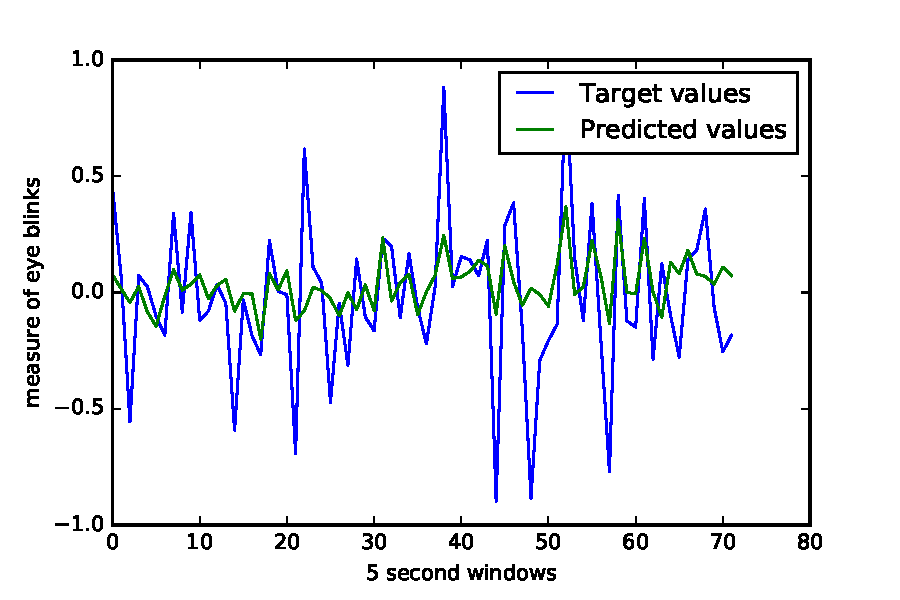
\includegraphics[width=0.4\textwidth]{f1.pdf}
\caption{\label{fig:f1}Plot for Simon Video with SVR and size 200.}
\end{figure} 

\subsubsection{Full Audience and Feature Selection with Correlation-analysis}

The follwing $R^2$ results were obtained for given reduced acoustic dataset sizes. Table~\ref{tab:carol2} gives results for Carol TEDx video and Table~\ref{tab:simon2} for Simon TEDx video. Figure~\ref{fig:f2} shows the plot for the best result obtained here.

\begin{table}
\centering
\begin{tabular}{ |p{3cm}||p{3cm}|p{3cm}|p{3cm}|  }
 \hline
 \multicolumn{3}{|c|}{$R^2 scores$} \\
 \hline
 Dataset Size &MLP &SVR\\
 \hline
 10 & 0.23 & 0.11\\
 20 & 0.47 & 0.44\\
 50 & 0.38 & 0.43\\
 100 & 0.26 & 0.48\\
 200 & 0.19 & 0.44\\
 \hline
\end{tabular}
\caption{\label{tab:carol2}Results for Carol Video.}
\end{table}

\begin{table}
\centering
\begin{tabular}{ |p{3cm}||p{3cm}|p{3cm}|p{3cm}|  }
 \hline
 \multicolumn{3}{|c|}{$R^2 scores$} \\
 \hline
 Dataset Size &MLP &SVR\\
 \hline
 10 & 0.31 & 0.21\\
 20 & 0.48 & 0.40\\
 50 & 0.54 & 0.45\\
 100 & 0.48 & 0.52\\
 200 & 0.45 & 0.55\\
 \hline
\end{tabular}
\caption{\label{tab:simon2}Results for Simon Video.}
\end{table}

\begin{figure}
\centering
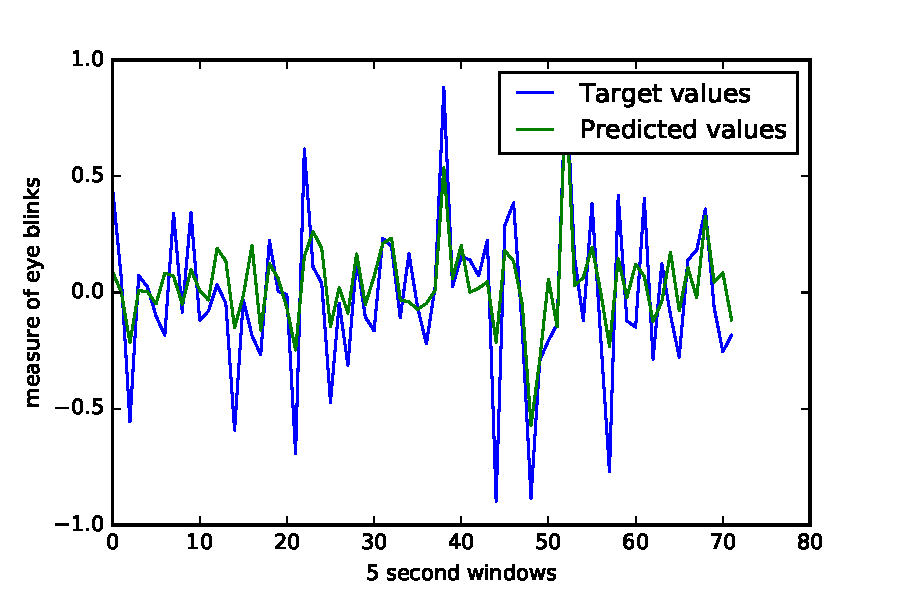
\includegraphics[width=0.4\textwidth]{f2.pdf}
\caption{\label{fig:f2}Plot for Simon Video with SVR and size 200.}
\end{figure} 

\subsubsection{Reduced Audience and Feature Selection with Eigen-analysis}

The follwing $R^2$ results were obtained for given reduced acoustic dataset sizes. Table~\ref{tab:carol3} gives results for Carol TEDx video and Table~\ref{tab:simon3} for Simon TEDx video. Figure~\ref{fig:f3} shows the plot for the best result obtained here.

\begin{table}
\centering
\begin{tabular}{ |p{3cm}||p{3cm}|p{3cm}|p{3cm}|  }
 \hline
 \multicolumn{3}{|c|}{$R^2 scores$} \\
 \hline
 Dataset Size &MLP &SVR\\
 \hline
 10 & -0.52 & 0.09\\
 20 & -0.03 & 0.28\\
 50 & -0.008 & 0.31\\
 100 & 0.03 & 0.32\\
 200 & -0.68 & 0.29\\
 \hline
\end{tabular}
\caption{\label{tab:carol3}Results for Carol Video.}
\end{table}

\begin{table}
\centering
\begin{tabular}{ |p{3cm}||p{3cm}|p{3cm}|p{3cm}|  }
 \hline
 \multicolumn{3}{|c|}{$R^2 scores$} \\
 \hline
 Dataset Size &MLP &SVR\\
 \hline
 10 & -0.32 & -0.114\\
 20 & 0.12 & 0.095\\
 50 & 0.26 & 0.14\\
 100 & 0.20 & 0.17\\
 200 & -0.17 & 0.16\\
 \hline
\end{tabular}
\caption{\label{tab:simon3}Results for Simon Video.}
\end{table}

\begin{figure}
\centering
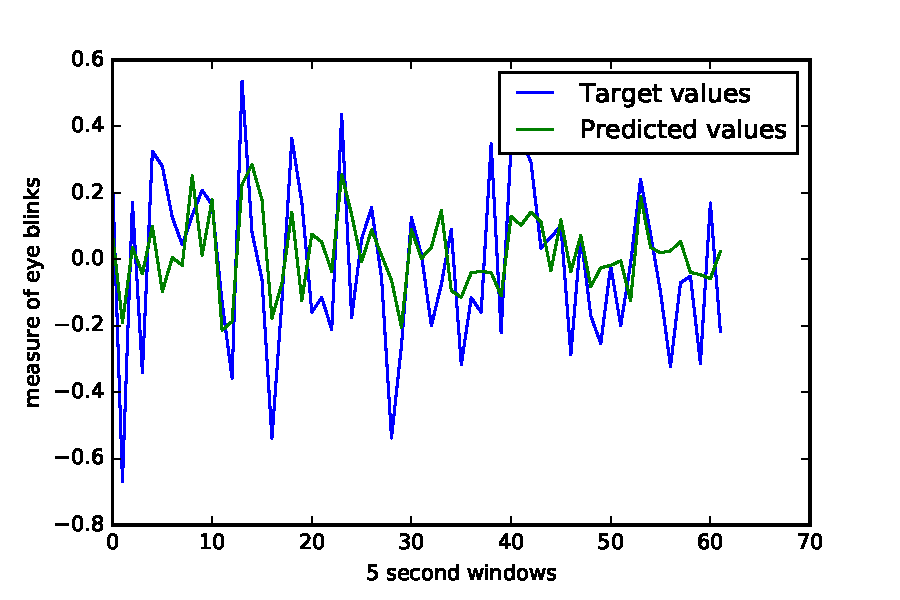
\includegraphics[width=0.4\textwidth]{f3.pdf}
\caption{\label{fig:f3}Plot for Carol Video with SVR and size 100.}
\end{figure} 

\subsubsection{Reduced Audience and Feature Selection with Correlation-analysis}

The follwing $R^2$ results were obtained for given reduced acoustic dataset sizes. Table~\ref{tab:carol4} gives results for Carol TEDx video and Table~\ref{tab:simon4} for Simon TEDx video. Figure~\ref{fig:f4} shows the plot for the best result obtained here.

\begin{table}
\centering
\begin{tabular}{ |p{3cm}||p{3cm}|p{3cm}|p{3cm}|  }
 \hline
 \multicolumn{3}{|c|}{$R^2 scores$} \\
 \hline
 Dataset Size &MLP &SVR\\
 \hline
 10 & 0.004 & 0.14\\
 20 & 0.34 & 0.40\\
 50 & 0.36 & 0.48\\
 100 & 0.39 & 0.51\\
 200 & 0.20 & 0.53\\
 \hline
\end{tabular}
\caption{\label{tab:carol4}Results for Carol Video.}
\end{table}

\begin{table}
\centering
\begin{tabular}{ |p{3cm}||p{3cm}|p{3cm}|p{3cm}|  }
 \hline
 \multicolumn{3}{|c|}{$R^2 scores$} \\
 \hline
 Dataset Size &MLP &SVR\\
 \hline
 10 & 0.27 & 0.34\\
 20 & 0.51 & 0.43\\
 50 & 0.47 & 0.52\\
 100 & 0.48 & 0.53\\
 200 & 0.51 & 0.57\\
 \hline
\end{tabular}
\caption{\label{tab:simon4}Results for Simon Video.}
\end{table}

\begin{figure}
\centering
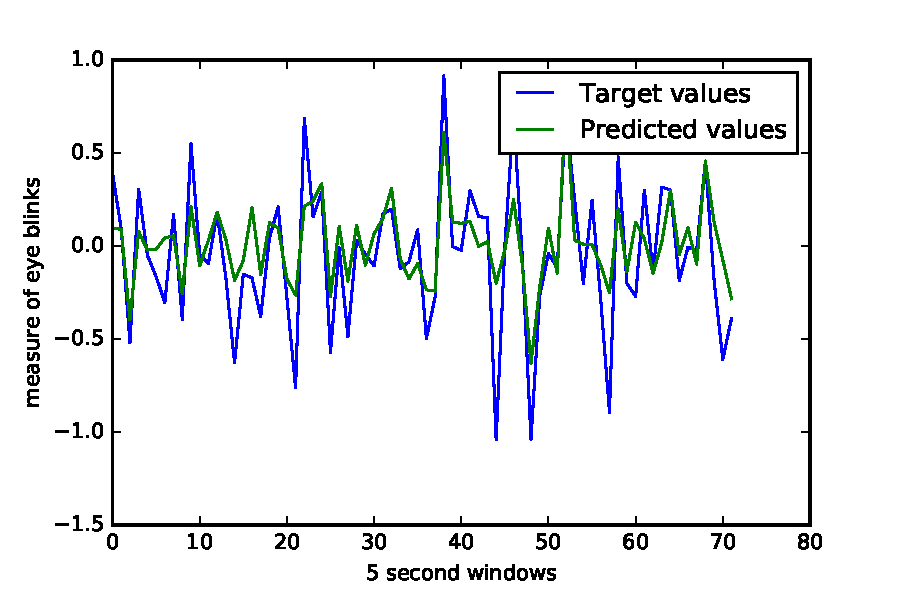
\includegraphics[width=0.4\textwidth]{f4.pdf}
\caption{\label{fig:f4}Plot for Simon Video with SVR and size 200.}
\end{figure} 

\subsubsection{Relevant Features with respect to Attention}
Only the correlation-analysis gave good results. Therefore the relevant features obtained through this feature selection were determined for both the full audience case and reduced one.

Top 10 features for Carol video with Full Audience:
\begin{itemize}
\item \verb|audspec_lengthL1norm_sma_stddev|:standard deviation of magnitude of the L1 norm of auditory spectrum and it was smoothed using an averaging filter with window length 3.
\item \verb|audSpec_Rfilt_sma[0]_range|:Rfilt means Relative Spectral Transform (RASTA)-style filtered. This means range of 0th Rfilt of auditory spectrum and it was smoothed using an averaging filter with window length 3.
\item \verb|audSpec_Rfilt_sma[19]_percentile1.0|:Rfilt means Relative Spectral Transform (RASTA)-style filtered. Percentile1.0 is the outlier-robust minimum value of the contour, represented by the 1 percentile. This means percentile1.0 of 19th Rfilt of auditory spectrum and it was smoothed using an averaging filter with window length 3.
\item \verb|audSpec_Rfilt_sma[24]_range|:Rfilt means Relative Spectral Transform (RASTA)-style filtered. This means range of 24th Rfilt of auditory spectrum and it was smoothed using an averaging filter with window length 3.
\item \verb|audSpec_Rfilt_sma[25]_percentile1.0|:Rfilt means Relative Spectral Transform (RASTA)-style filtered. Percentile1.0 is the outlier-robust minimum value of the contour, represented by the 1 percentile. This means percentile1.0 of 25th Rfilt of auditory spectrum and it was smoothed using an averaging filter with window length 3.
\item \verb|pcm_fftMag_spectralRollOff75.0_sma_leftctime|: The 75 ∗ 100 percent spectral roll-off point is determined as the frequency below which 75 ∗ 100 percent of the total signal energy fall. This means time during which the spectralRollOff75.0 of fast Fourier transformed pulse-code modulation has left curvature and it was smoothed using an averaging filter with window length 3.
\item \verb|mfcc_sma[2]_range|:range of 2nd mel-frequency cepstral coefficient and it was smoothed using an averaging filter with window length 3.
\item \verb|mfcc_sma[4]_percentile1.0|:Percentile1.0 is the outlier-robust minimum value of the contour, represented by the 1 percentile. This means percentile1.0 of 4th mel-frequency cepstral coefficient and it was smoothed using an averaging filter with window length 3.
\item \verb|mfcc_sma[8]_percentile99.0|:Percentile99.0 is the outlier-robust maximum value of the contour, represented by the 99 percentile. This means percentile99.0 of 8th mel-frequency cepstral coefficient and it was smoothed using an averaging filter with window length 3.
\item \verb|mfcc_sma_de[4]_range|:range of 4th mel-frequency cepstral coefficient and it was smoothed using an averaging filter with window length 3.
\end{itemize}

Top 10 features for Simon video with Full Audience:
\begin{itemize}
\item \verb|pcm_zcr_sma_percentile99.0|:Percentile99.0 is the outlier-robust maximum value of the contour, represented by the 99 percentile. This means percentile99.0 of zero-crossing rate of time signal and it was smoothed using an averaging filter with window length 3.
\item \verb|audspec_lengthL1norm_sma_de_range|:range of magnitude of the L1 norm of auditory spectrum and it was smoothed using an averaging filter with window length 3.
\item \verb|audSpec_Rfilt_sma[9]_range|:Rfilt means Relative Spectral Transform (RASTA)-style filtered. This means range of 9th Rfilt of auditory spectrum and it was smoothed using an averaging filter with window length 3.
\item \verb|audSpec_Rfilt_sma[15]_range|:Rfilt means Relative Spectral Transform (RASTA)-style filtered. This means range of 15th Rfilt of auditory spectrum and it was smoothed using an averaging filter with window length 3.
\item \verb|audSpec_Rfilt_sma[16]_pctlrange0-1|:Rfilt means Relative Spectral Transform (RASTA)-style filtered. This means 0-1 inter-percentile range of 16th Rfilt of auditory spectrum and it was smoothed using an averaging filter with window length 3.
\item \verb|pcm_fftMag_spectralRollOff25.0_sma_range|: The 25 ∗ 100 percent spectral roll-off point is determined as the frequency below which 25 ∗ 100 percent of the total signal energy fall. This means range of spectralRollOff25.0 of fast Fourier transformed pulse-code modulation and it was smoothed using an averaging filter with window length 3.
\item \verb|pcm_fftMag_spectralHarmonicity_sma_range|:A Harmonicity object represents the degree of acoustic periodicity, also called Harmonics-to-Noise Ratio (HNR). This means range of spectral harmonicity of fast Fourier transformed pulse-code modulation and it was smoothed using an averaging filter with window length 3.
\item \verb|audSpec_Rfilt_sma_de[8]_range|:Rfilt means Relative Spectral Transform (RASTA)-style filtered. This means range of 8th Rfilt of auditory spectrum and it was smoothed using an averaging filter with window length 3.
\item \verb|pcm_fftMag_spectralSlope_sma_peakRangeAbs|:absolute value of range of all values for spectral slope of fast Fourier transformed pulse-code modulation and it was smoothed using an averaging filter with window length 3.
\item \verb|audspec_lengthL1norm_sma_de_peakRangeAbs|:absolute value of range of all values for magnitude of the L1 norm of auditory spectrum and it was smoothed using an averaging filter with window length 3.
\end{itemize}

Top 10 features for Carol video with Reduced Audience:
\begin{itemize}
\item \verb|audspec_lengthL1norm_sma_quartile2|:$50th$ percentile of magnitude of the L1 norm of auditory spectrum and it was smoothed using an averaging filter with window length 3.
\item \verb|pcm_RMSenergy_sma_percentile99.0|:Percentile99.0 is the outlier-robust maximum value of the contour, represented by the 99 percentile. This means percentile99.0 of root-mean-square signal frame energy and it was smoothed using an averaging filter with window length 3.
\item \verb|pcm_RMSenergy_sma_pctlrange0-1|:This means 0-1 inter-percentile range of root-mean-square signal frame energy and it was smoothed using an averaging filter with window length 3.
\item \verb|audSpec_Rfilt_sma[20]_percentile1.0|:Rfilt means Relative Spectral Transform (RASTA)-style filtered. Percentile1.0 is the outlier-robust minimum value of the contour, represented by the 1 percentile. This means percentile1.0 of 20th Rfilt of auditory spectrum and it was smoothed using an averaging filter with window length 3.
\item \verb|mfcc_sma[1]_percentile99.0|:Percentile99.0 is the outlier-robust maximum value of the contour, represented by the 99 percentile. This means percentile99.0 of 1st mel-frequency cepstral coefficient and it was smoothed using an averaging filter with window length 3.
\item \verb|audSpec_Rfilt_sma_de[23]_percentile99.0|:Rfilt means Relative Spectral Transform (RASTA)-style filtered. Percentile99.0 is the outlier-robust maximum value of the contour, represented by the 99 percentile. This means percentile99.0 of 25th Rfilt of auditory spectrum and it was smoothed using an averaging filter with window length 3.
\item \verb|audSpec_Rfilt_sma[6]_meanRisingSlope|:meanRisingSlope is the mean of rising slopes, i.e. the slopes connecting a valley with the following peak. Rfilt means Relative Spectral Transform (RASTA)-style filtered. This means meanRisingSlope of 6th Rfilt of auditory spectrum and it was smoothed using an averaging filter with window length 3.
\item \verb|pcm_fftMag_spectralRollOff50.0_sma_minRangeRel|:The 50 ∗ 100 percent spectral roll-off point is determined as the frequency below which 50 ∗ 100 percent of the total signal energy fall. This means minimum value of relative range of spectralRollOff50.0 of fast Fourier transformed pulse-code modulation and it was smoothed using an averaging filter with window length 3.
\item \verb|audSpec_Rfilt_sma_de[21]_peakMeanAbs|:Rfilt means Relative Spectral Transform (RASTA)-style filtered. This means absolute value of mean of all values for 21th Rfilt of auditory spectrum and it was smoothed using an averaging filter with window length 3.
\item \verb|audSpec_Rfilt_sma_de[21]_peakMeanMeanDist|:Rfilt means Relative Spectral Transform (RASTA)-style filtered. This means mean of distance between peaks for 21th Rfilt of auditory spectrum and it was smoothed using an averaging filter with window length 3.
\end{itemize}

Top 10 features for Simon video with Reduced Audience:
\begin{itemize}
\item \verb|audSpec_Rfilt_sma[13]_range|:Rfilt means Relative Spectral Transform (RASTA)-style filtered. This means range of 13th Rfilt of auditory spectrum and it was smoothed using an averaging filter with window length 3.
\item \verb|audSpec_Rfilt_sma[23]_range|:Rfilt means Relative Spectral Transform (RASTA)-style filtered. This means range of 23th Rfilt of auditory spectrum and it was smoothed using an averaging filter with window length 3.
\item \verb|pcm_fftMag_spectralRollOff25.0_sma_percentile99.0|:Percentile99.0 is the outlier-robust maximum value of the contour, represented by the 99 percentile. The 25 ∗ 100 percent spectral roll-off point is determined as the frequency below which 25 ∗ 100 percent of the total signal energy fall. This means percentile99.0 of spectralRollOff25.0 of fast Fourier transformed pulse-code modulation and it was smoothed using an averaging filter with window length 3.
\item \verb|pcm_fftMag_spectralFlux_sma_range|:range of spectral flux of fast Fourier transformed pulse-code modulation and it was smoothed using an averaging filter with window length 3.
\item \verb|pcm_fftMag_spectralSkewness_sma_range|:Spectral skewness is a measure of the asymmetry of the spectral distribution around its centroid. This means range of spectral skewness of fast Fourier transformed pulse-code modulation and it was smoothed using an averaging filter with window length 3.
\item \verb|pcm_fftMag_psySharpness_sma_percentile1.0|:psySharpness is related to how much a sound’s spectrum is in the high end. Percentile1.0 is the outlier-robust minimum value of the contour, represented by the 1 percentile. This means percentile1.0 of psySharpness of fast Fourier transformed pulse-code modulation and it was smoothed using an averaging filter with window length 3.
\item \verb|mfcc_sma[6]_percentile1.0|:Percentile1.0 is the outlier-robust minimum value of the contour, represented by the 1 percentile. This means percentile1.0 of 6th mel-frequency cepstral coefficient and it was smoothed using an averaging filter with window length 3.
\item \verb|audSpec_Rfilt_sma_de[20]_range|:Rfilt means Relative Spectral Transform (RASTA)-style filtered. This means range of 20th Rfilt of auditory spectrum and it was smoothed using an averaging filter with window length 3.
\item \verb|pcm_fftMag_spectralFlux_sma_de_range|:delta of range of spectral flux of fast Fourier transformed pulse-code modulation and it was smoothed using an averaging filter with window length 3.
\item \verb|audSpec_Rfilt_sma_de[5]_stddevRisingSlope|:stddevRisingSlope is the standard deviation of rising slopes, i.e. the slopes connecting a valley with the following peak. Rfilt means Relative Spectral Transform (RASTA)-style filtered. This means stddevRisingSlope of 5th Rfilt of auditory spectrum and it was smoothed using an averaging filter with window length 3.
\end{itemize}

\section{Conclusion}

Best results were obtained using the correlation based feature selection for both the full audience and reduced audience case. For the full audience experiment, the best results were obtained for Simon video with SVR and correlation based feature selection of 200 features. Again for reduced dataset experiment, the best results were obtained for Simon video with SVR and correlation based feature selection of 200 features. The SVR learning method consistently out-performed the MLP method. 

The relevant audio features were also obtained for both the experiments. Future work can include further interpretation of the relevant features obtained. Also some other audio feature extraction methods can be explored. 


\begin{thebibliography}{9}
\bibitem{political} 
Zhang, John R., et al.
\textit{Correlating Speaker Gestures in Political Debates with Audience Engagement Measured via EEG}. 
Proceedings of the ACM International Conference on Multimedia. ACM, 2014.

\bibitem{opensmile} 
Eyben, Florian, Martin Wllmer, and Bjrn Schuller.
\textit{Opensmile: the munich versatile and fast open-source audio feature extractor}. 
Proceedings of the international conference on Multimedia. ACM, 2010.

\bibitem{compare} 
Schuller, Bjrn, et al.
\textit{The INTERSPEECH 2013 computational paralinguistics challenge: social signals, conflict, emotion, autism}. 
(2013).

\bibitem{audio} 
Eyben, Florian, et al.
\textit{The acoustics of eye contact: detecting visual attention from conversational audio cues}. 
Proceedings of the 6th workshop on Eye gaze in intelligent human machine interaction: gaze in multimodal interaction. ACM, 2013.

\bibitem{ffmpeg} 
Bellard, Fabrice, and M. Niedermayer.
\textit{FFmpeg}. 
http://ffmpeg.org (2012).

\bibitem{scikit} 
Pedregosa et al.
\textit{Scikit-learn: Machine Learning in Python}. 
JMLR 12, pp. 2825-2830, 2011.

\bibitem{nn} 
M.W.Gardener, S.R. Dorling.
\textit{ARTIFICIAL Neural Networks(The Multilayer perceptron)- A review of the applications in Atmospheric Sciences}. 
June 1998.

\bibitem{bp} 
Christopher Bishop.
\textit{Pattern Recognition and Machine Learning}. 
book, (2007).

\bibitem{svr} 
Alex J. Samola, Bernard S.
\textit{A tutorial on Support Vector Regression}. 
NeuroCOLT2 Technical Report NCR2, October 1998.

\end{thebibliography}

%\bibliography{references}

\end{document}